\section{one dimension}

\begin{comment}
 Outline:
1. T/${\cal E}$ as a criteria
  a. motivation
  b. why other criteria won't suffice
2. diffusive system
  a. solve diffusive equ analytically for slab with gain, 
       and we know diffusive system doesn't apply to localization
  b. find T, E. Plot a function of gain, L
  c. T/${\cal E}$ looks to be constant
  d. diffusion equation doesn't account for phase, which is the cause of localization
3. 1-D localization
  a. Setup: 1-D passive random system of alternating layers
  b. Results: peaks match/mismatch: T/${\cal E}$ is not smooth
  c. analysis: tunneling - look at analytical models
     i. double barrier potential 
     ii. periodic layers with single defect
  d. math analysis: energy is stored
  e. add gain
  f. closed system
  g. math reasoning, quantum well
  h. look for det[] = 0
  i. add gain
4. conclusion
5. future work

\end{comment}

%%%%%%%%%%%%%%%%%%%%%%%%%%%%%%%%%%%%%%%%%%%%%%%%%%%%%%%%%
\subsection {Motivation: T/${\cal E}$ as a parameter for localization with gain}
%%%%%%%%%%%%%%%%%%%%%%%%%%%%%%%%%%%%%%%%%%%%%%%%%%%%%%%%%

Localization criteria developed for passive systems may not be applicable for random media with gain. Transmission coefficients and the magnitude of their fluctuations diverge close to lasing threshold. In realistic systems, saturation prevents the divergence but introduces the dependence on saturation parameter. This may not carry the desired information about wave transport.

The Thouless criteria may not account for gain: % see NSF proposal, top of page 5,7
``The ensemble-averaged spectral correlation function might be dominated by the rare lasing configurations, thus the spectral correlation width could be equal to the lasing line width that depends on the properties of the gain material.'' [From NSF proposal.] [Need more background from NSF paper.] (Ioffe-Regel will not work in systems with gain?)

We confirm that transmission (T) and energy (${\cal E}$) both diverge as critical gain is approached in diffusive systems.  Either transmission~\cite{2000_chabanov_nature} or energy alone is not useful at critical gain, but perhaps a ratio of the two (T/${\cal E}$) will be non-divergent.

% what does the absorption model predict about resonant
% frequencies, standing waves, reciprocity?
% Perhaps we can extend our model to the absorption regime also?

%%%%%%%%%%%%%%%%%%%%%%%%%%%%%%%%%%%%%%%%%%%%%%%%%%%%%%%%%
\subsection {Diffusion: Slab geometry}
%%%%%%%%%%%%%%%%%%%%%%%%%%%%%%%%%%%%%%%%%%%%%%%%%%%%%%%%%

In starting to look for criteria for localization in systems with gain we first looked at diffusive systems. The reason for starting out in the diffusive model is because the diffusion equation can be solved analytically for the slab geometry, even when gain is added~\cite{1993_Lisyansky_diffusint}. We need to see how light is transmitted through media in general. 

We know there will not be any strong localization in systems described by the diffusion equation since the model does not keep track of phase.  Localization is based on interaction of waves and this interference is dependent on the phase.  Any model that does not account for phase or some derivative of phase will not be able to fully account for strong localization.

Gain cannot always be modelled by negative absorption. Close to lasing threshold the phase (i.e description of fields not intensities), fluctuations and the system dynamics become important. Far from lasing threshold, ``negative absorption'' is a reasonable way of introducing gain.
%Gain will be incorporated by adding an imaginary component to the dielectric constant.

Starting from the intensity distribution from Ref.~\cite{2004_Yamilov_intensity} we can find the transmission and reflection from Eq.~\ref{eq:diffusionequ}
\begin{equation}
J _{\pm} = \frac{c}{4} I \mp \frac{D}{2} \frac{dI}{dz}
\label{eq:diffusionequ}
\end{equation}
where $ J _- $ is the reflection flux, $ J _+ $ is the transmission flux, $I(z)$ is the intensity, and z is the position within the slab. Substituting the expression for $I(z)$ found in Ref.~\cite{diffusint}, we find
\begin{equation}
J _- (0) = \frac{c}{4} \frac{2 z _o q}{D} \\
\frac{\sinh(\alpha  (L-z _p)) + \alpha z_o \cosh(\alpha (L-z _p))}{\\
(1+ \alpha ^2 z_o ^2) \sinh(\alpha L) + 2 \alpha z_o \cosh(\alpha L)}
\label{eq:Jreflectionflux}
\end{equation}
and
\begin{equation}
J _+ (L) = \frac{c}{4} \frac{2 z _o q}{D} \\
\frac{\sinh(\alpha z_p) + \alpha z _o \cosh(\alpha z_p)}{(1+\alpha^2 z_o^2) \sinh(\alpha L) + 2 \alpha z_o \cosh(\alpha L)}
\label{eq:Jtransmissionflux}
\end{equation}
where $ J _{incident} = q $. We can also find the energy by integrating intensity over the entire system:
\begin{equation}
{\cal E} = \frac{q}{4 \pi D \alpha ^2} \left(1-\frac{\sinh(\alpha z_p) + \\
\sinh(\alpha (L-z_p))+\alpha z_o (\cosh(\alpha z_p) + \\
\cosh(\alpha (L - z_p))}{\sinh(\alpha L (1+\alpha^2 z_o^2))+\\
\cosh(\alpha L 2 \alpha z_o)}\right)
\label{fig:Jenergy}
\end{equation}
We plot transmission, Eq.~\ref{eq:Jtransmissionflux},and reflection, Eq.~\ref{eq:Jreflectionflux}, with and without normalization by energy ${\cal E}$, Eq.~\ref{fig:Jenergy}, as functions of gain and absorption in Fig.~\ref{fig:diffusiveRTRETE}.  
\begin{figure}
\vskip -0.5cm
\centerline{
\scalebox{0.4}{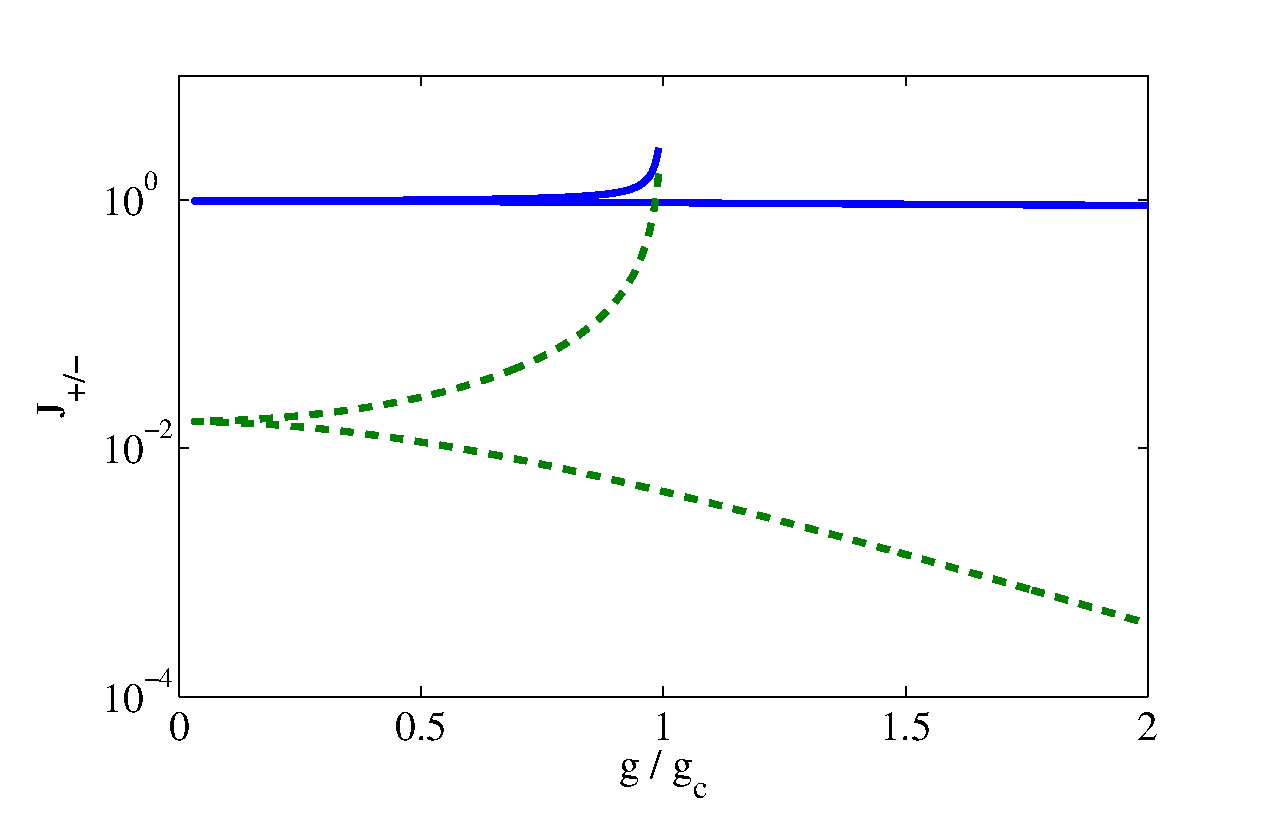
\includegraphics{pictures/yamilov_fixed_L_variable_gain_R_T}}
\scalebox{0.4}{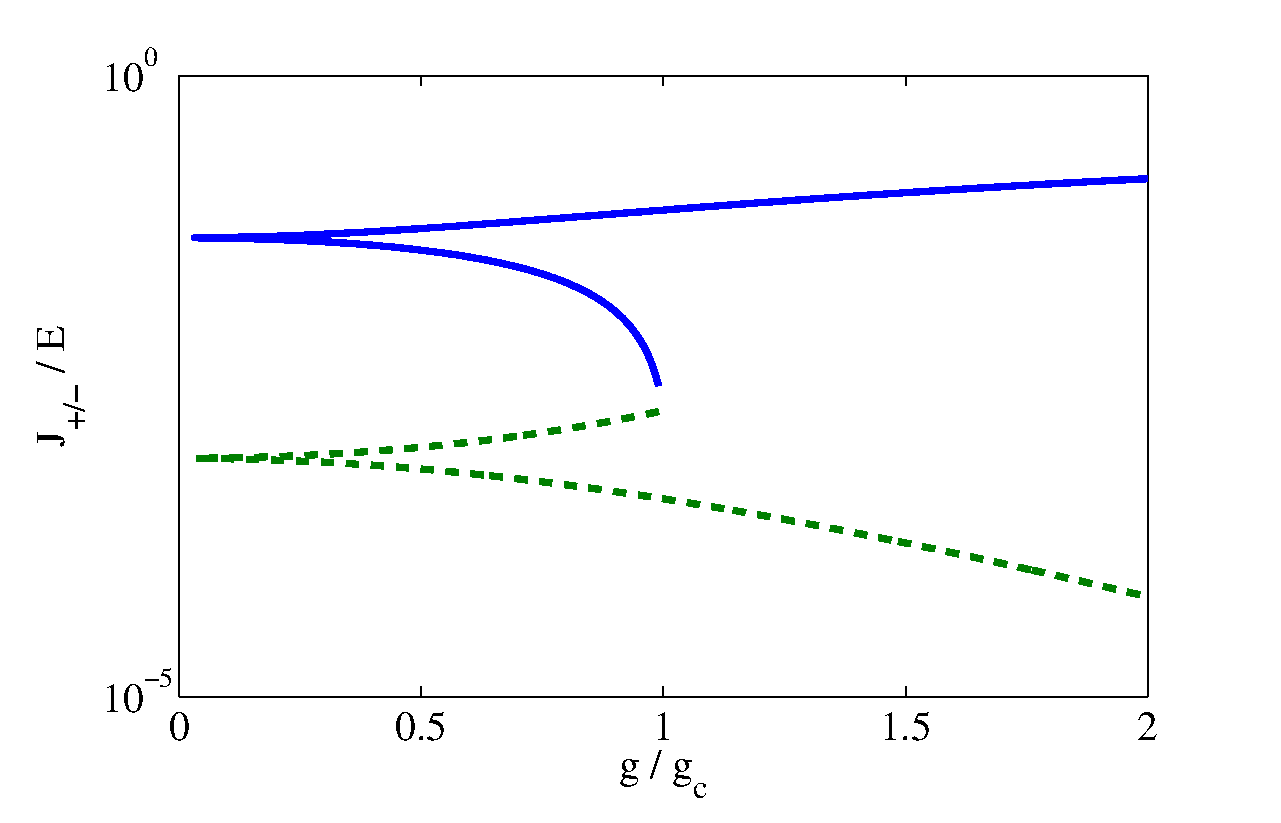
\includegraphics{pictures/yamilov_fixed_L_variable_gain_R_T_divided_by_Energy}}
}
\vskip -0.5cm
\caption[Transmission and reflection are plotted for increasing gain and absorption coefficients.]{Transmission and reflection are plotted for increasing gain and absorption coefficients. In the left plot dotted green line is transmission and solid line blue is reflection. In the left plot the upper dotted green and upper solid blue lines are transmission and reflection with increasing amounts of gain, both diverging at the critical gain value. The lower dotted green and lower solid blue lines are absorption.  In the right plot we see transmission/energy and reflection/energy.  Now when gain is added neither T/${\cal E}$ (upper dotted green line) nor R/${\cal E}$ (lower solid blue line) diverge at critical gain, and they both reach the same value. T/${\cal E}$ (lower dotted green line) and R/${\cal E}$ (upper solid blue line) in the absorption regime do nothing unexpected.}
\label{fig:diffusiveRTRETE}
\end{figure}

As critical gain is reached both transmission and reflection diverge asymptotically in Fig.~\ref{fig:diffusiveRTRETE} a according to
\begin{equation}
q \frac{z_o + z_p}{\pi} \frac{\alpha _c ^2}{\alpha _c - \alpha}
\end{equation}

Plotting the ratios of reflection to energy $( \frac{J_-}{\cal E} ) $
and transmission to energy $( \frac{J_+}{\cal E} ) $ in Fig.~\ref{fig:diffusiveRTRETE}
we see two things: T/${\cal E}$ does not diverge at critical gain, and the ratios 
of R/${\cal E}$ and T/${\cal E}$ match
at the critical gain. This tells us that T/${\cal E}$ may be a good
criteria for detecting localization (whereas both T and
R are divergant at critical gain).  Note that although
R/${\cal E}$ doesn't diverge, we don't use it because transmission may be 
easier to measure.

Another method for reaching a lasing state is to have a certain
amount of gain for a material and then adjust the length of the
sample until a critical length is reached such that the leakage
(this is an open system) is compensated by the cumulative
effect of the gain in the material. We see similar behavior
for the reflection and transmission (divergence of both transmission
and reflection in systems
near the critical length) versus R/${\cal E}$ and T/${\cal E}$ ratios (both converge
to same value at critical gain, both are non-divergent) in this
alternate analytical diffusion model.

The last thing we investigate in the diffusive system
is how the distribution of the intensity in the sample changes
for active systems and systems with absorption. When gain
is added there is more energy stored in the sample, as compared
to the passive and absorption regimes. See
Fig.~\ref{fig:diffusiveIntensityDistribution}. We also see that the intensity
decreases as it passes through the sample. If light were
shined on the other side of the sample we would see the decay
in intensity flip (decreasing from a maxium at x=L to near
zero at x=0).

\begin{figure}
\vskip -0.5cm
\centerline{\scalebox{0.4}{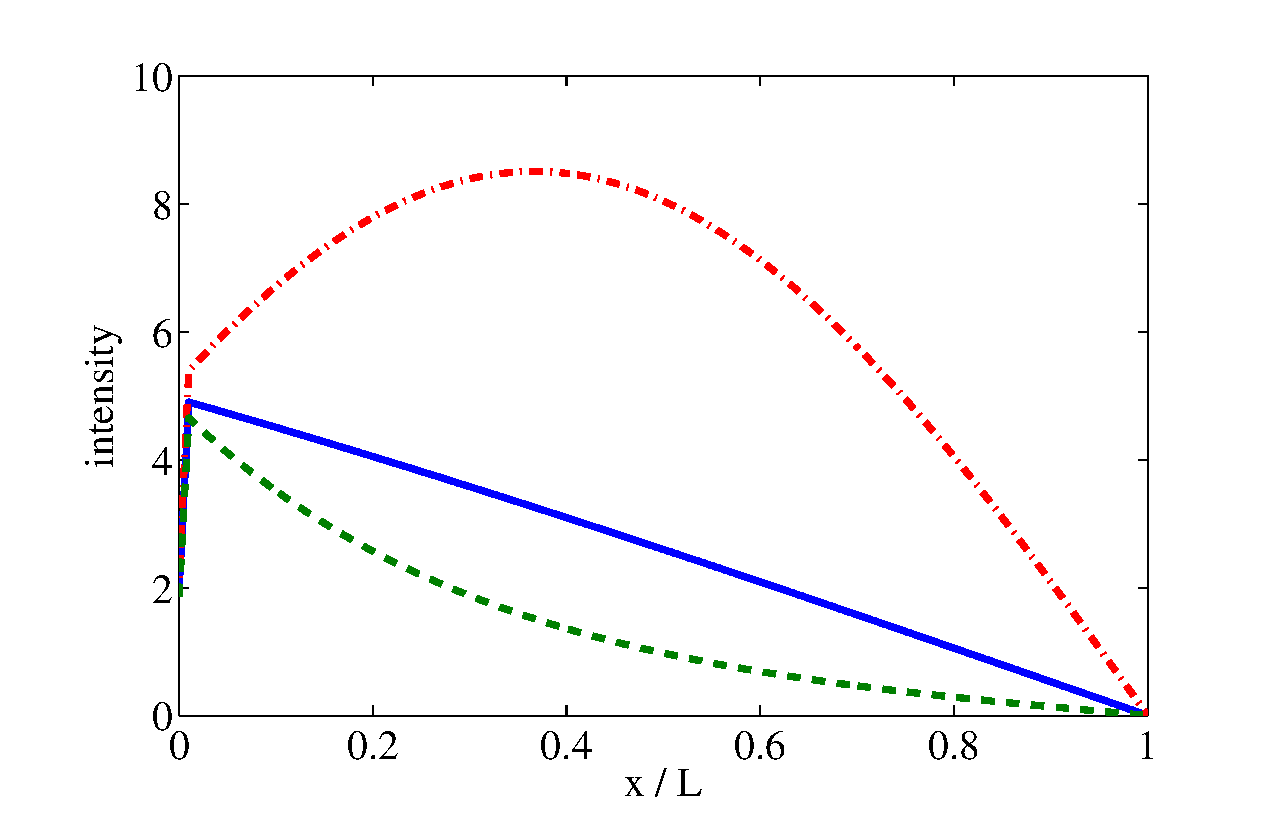
\includegraphics{pictures/yamilov_diffusive_intensity_distribution}}}
\vskip -0.5cm
\caption[Intensity distribution for the diffusive system.]{Intensity distribution for the diffusive system. Top red dotted line is 
the sample with gain, middle solid blue line is passive sample, lower dotted green line
is sample in the absorption regime. We can see that the amount of gain or absorption in the sample affects the field in the sample. This is verified in non-diffusive models.}
\label{fig:diffusiveIntensityDistribution}
\end{figure}

%%%%%%%%%%%%%%%%%%%%%%%%%%%%%%%%%%%%%%%%%%%%%%%%%%%%%%%%%
\subsection {Localization: stacks of dielectric layers model}
%%%%%%%%%%%%%%%%%%%%%%%%%%%%%%%%%%%%%%%%%%%%%%%%%%%%%%%%%

\subsubsection{Description of Setup}

We consider a passive system having layers of alternating ($\epsilon = 1$ and $1.2$) dielectric material, resulting in alternating refractive index ($n = \sqrt{\epsilon}$). This pair of layers is repeated to create 1000 pairs. One last $\epsilon = 1$ layer is added to the end to create a symmetric stack of 2001 layers. Then the total sample has length L. Randomness is introduced by varying the width of each $\epsilon=1.2$ layer. The variance of the random layers is such that localization length is between L/2 and L/5. Gain or absorption can be arbitrarily added by changing the value of the dielectric to be complex or negative, respectively, (but not both). Fig.~\ref{fig:dimaSetup} schematically shows the setup. These parameters put the model in the localization regime ($a\ll\lambda\ll L$). [What is a?] Where $\lambda$=wavelength, L is system length. The frequency range is chosen so that single parameter scaling is satisfied. [citation?]

\begin{figure}
\vskip -0.5cm
\centerline{\scalebox{0.8}{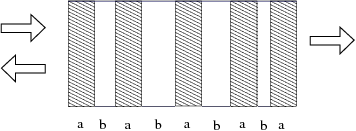
\includegraphics{pictures/dima_setup_cartoon}}}
\vskip -0.5cm
\caption[Layer setup for alternating pairs of dielectric.]{Layer setup for alternating pairs of dielectric. %``A'' and ``B'' form a pair.  
Solid blue layer A has a constant width, while the width of B has uniformly random variance of width between 1.1 and .9.  Light is incident on the left side of the sample with amplitude 1. Some light is reflected to the left and some is transmitted to the right.}
\label{fig:dimaSetup}
\end{figure}

Light is shone on one side of the material (from left to right) and the propagation of the light through the sample is calculated using Maxwell's equations and the transfer matrix method. The transfer matrix method is covered in detail around page 44 in a text book by Mello and Kumar\cite{2004_Mello_Kumar_book}. See also Appendix A.
% starting at equation 2.165
% see also notes 20080127
As a check, the magnitude of transmission and reflection add to one is verified.

% too technical
\begin{comment}
We multiply 2x2 matrices together (for 2001 layers). However, because of rounding error (using fortran 90) we need to use self-embedding technique~\cite{1999_yamilov_selfembed}. This means doing 200 matrix multiplications (resulting in a single 2x2 matrix) and then multiplying that by the next 200 matrices. Repeat for a total of five chunks. No re-normalization of the 2x2 matrices is necessary.

The amount of numerical data of this one-dimensional system scales with the number of layers (2001). Usually one considers many frequencies and/or many realizations. The results give managable dataset sizes (on the order of Megabytes) and the computational time is on the order of minutes.
\end{comment}

Using the computational model the cumulative energy in the system and the transmission are found for a given frequency. Then we scan many frequencies. Then in order to get generalized behavior we alter the random widths to produce another sample. Repeat to find ensemble behavior. 

We chose not to take any averages; rather we look at a single realization of disorder and attempt to understand it. Once the behavior is understood for a single instance we can develop a general phenomenological explaination.

\begin{figure}
\vskip -0.5cm
\centerline{\scalebox{0.5}{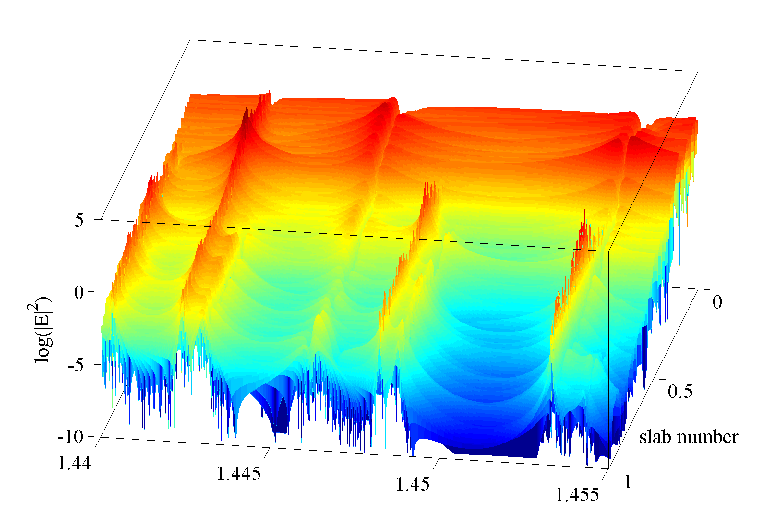
\includegraphics{pictures/electric_field_in_sample}}}
\vskip -0.5cm
\caption[The log of electric field in a random sample for a range of frequencies versus position in the sample.]{The log of electric field in a random sample for a range of frequencies versus position in the sample. Without localization pure exponential decay is expected. This can be seen between $\omega$ =  1.45 and 1.453 as a straight line descending from the incident side at x/L=0 down to a minimum at x/L=1. Everywhere else in the sample localization effects are observed. At $\omega$ = 1.4425 a peak higher than the incident value can be seen. This would correspond to Fig. \ref{fig:onequarterthreequarterelecfield}a. At $\omega$ = 1.4475 there is an intial linear decline, then a peak, then further linear decline  (exponential decay), similar to Fig.~\ref{fig:onequarterthreequarterelecfield}b. A 2-D version of this plot can be seen in~\cite{2006_Genack_1d}.}
\label{fig:electricFieldInSample}
\end{figure}

This computational configuration has been realized experimentally with one dimensional experiments using microwaves by Genack~\cite{2006_Genack_1d}, Luna-Acosta~\cite{2008_LunaAcosta} and John Scales~\cite{2006_Scales}. Fig.~\ref{fig:electricFieldInSample} is the electric field plotted on a log scale for many frequencies. The electric field is related to the energy distribution in the sample.  [Explain importance, compare to Genack Nov 07 paper]

%%%%%%%%%%%%%%%%%%%%%%%%%%%%%%%%%%%%%%%%%%%%%%%%%%%%%%%%%
\subsubsection {Results for Passive Random Layers Model}
%%%%%%%%%%%%%%%%%%%%%%%%%%%%%%%%%%%%%%%%%%%%%%%%%%%%%%%%%

From the computational model we see peaks in transmission do not always have the corresponding peaks in energy (Fig.~\ref{fig:tenkenergytransmission}). We will call the frequencies for which transmission peaks occur resonant frequencies. From this plot of transmission and energy versus frequency we can tell that the ratio T/${\cal E}$ is not going to be flat since there are spikes in transmission that do not have the counterpart in energy.

\begin{figure}
\vskip -0.5cm
\centerline{\scalebox{0.5}{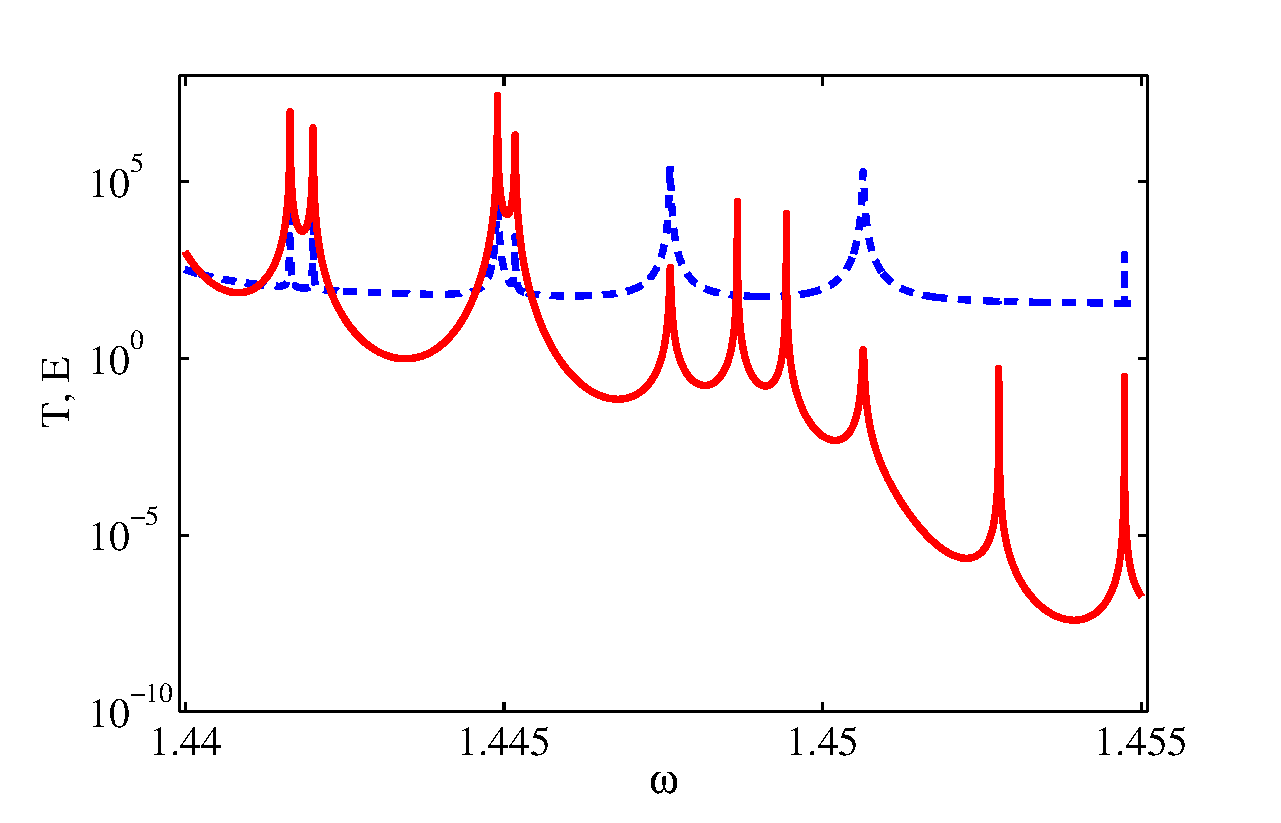
\includegraphics{pictures/tenk_energy_transmission_v_freq}}}
\vskip -0.5cm
\caption[Transmission as a function of frequency (omega) is compared to the total energy in the sample.]{Transmission as a function of frequency (omega) is compared to the total energy in the sample. This single represenative realization demonstrates that T/${\cal E}$ in the passive system will not be smooth. Transmission and energy sometimes share peaks for certain frequencies, but some peaks in transmission have no decernable peak in energy (even on a log plot with no noise).
%for left-to-right illumination.
}
\label{fig:tenkenergytransmission}
\end{figure}

% SIDE NOTE on A and B
Another quantity we can calculate in our computational model (in addition to the electric field and its derivative) is the amplitudes of the left and right traveling waves: A and B. Electric field in each layer is
\begin{equation}
\begin{gathered}
{\cal E}(x) = A \exp(i k n x) + B \exp(-i k n x) \\
A = \frac{1}{2} (E - i \frac{1}{k} \frac{dxi}{dx}) \\
B = \frac{1}{2} (E + i \frac{1}{k} \frac{dE}{dx})
\end{gathered}
\end{equation}
For resonant frequencies $ \| A \| \simeq \| B \| $ , which implies that it is almost like a standing wave with very little energy leakage, which is expected.

%                      For off resonant frequencies...(I don't have a plot of the A and B.)
% END SIDE NOTE

If the light is incident on the same sample but from the other side (ie right-to-left orientation) we see a different plot for transmission and energy versus frequency. Again, some peaks in transmission have no corresponding peak in energy while others do.

[Need a T, ${\cal E}$ v. freq plot showing RL is different]

Fluctuating T/${\cal E}$ is not of a significant concern, since we are in the passive system but the fact that it depends on illumination (from left of from right) is. % need to explain this concern more
It means that if we use this as a criterion, we will get a different value depending on how we perform the measurement. We will pay attention to this fact when we introduce the gain.

We investigate what is going on at those peak transmission frequencies. We would like to know why some peaks in transmission have corresponding peaks in energy while others do not. We also notice there are no cases where a peak in energy occurs and not transmission.

First, we confirm that for off-resonant frequencies we see exponential decay of the electric field through the sample. This is expected for random media in localization regime. When the exponential decay is plotted on a log scale we get a straight line.

Now we pick one resonant frequency and plot the electric field in the system. This is equivalent to looking at the energy inside the system. 
\begin{figure}
\vskip -0.5cm
\centerline{
\scalebox{0.4}{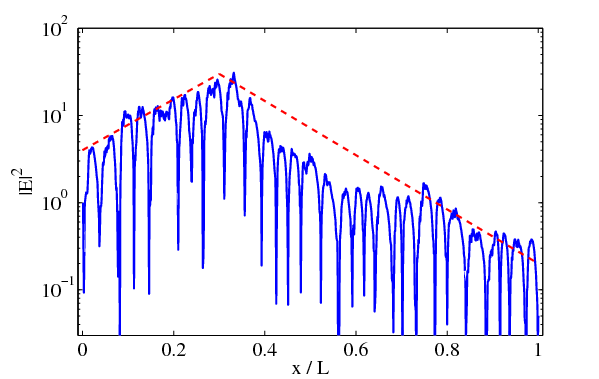
\includegraphics{pictures/rlz1_elecfield_14}}
\scalebox{0.4}{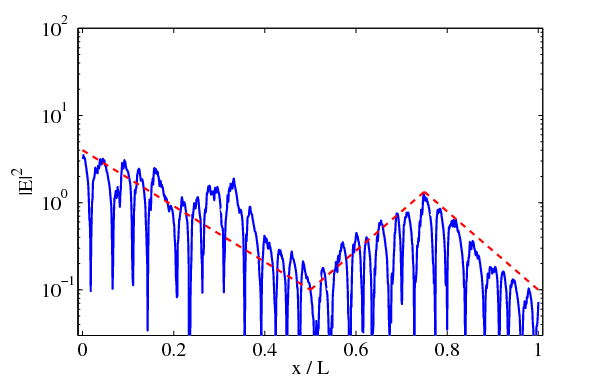
\includegraphics{pictures/rlz1_elecfield_34}}}
\vskip -0.5cm
\caption[In the left plot of the electric field (which is proportional to the energy stored in the sample) in the random media at resonant frequencies on a log scale there is a maximum near $ \frac{L}{4}$.]{In the left plot of the electric field (which is proportional to the energy stored in the sample) in the random media at resonant frequencies on a log scale there is a maximum near $ \frac{L}{4}$. This means there was exponential growth to the  center of localization, followed by exponential decay. The ratio of the amplitude at x=0 to x=L is approximately equal to the transmission. In the right plot we see a peak in electric field (energy) at $ \frac{3L}{4} $. For light to reach the center of localization  the light first exponentially decays, then grows, and falls again. The red dotted lines are the estimated slopes, which correspond to $\exp(\pm x/\xi)$.} 
\label{fig:onequarterthreequarterelecfield}
\end{figure}

Based on our analysis of many peaks in transmission, we conclude:
(i) At the frequencies where peaks in transmission 
and energy occur together there is a center of localization at $ 0 < x < \frac{L}{2}$. 
(ii) Where there is no corresponding peak in energy 
for a peak in transmission the center of localization occurs $ \frac{L}{2}<x<L $. 
We will use examples where the center of localization
happens at $ \frac{1}{4} $L, $ \frac{1}{2} $L, 
and $ \frac{3}{4} $L as canonical centers of localization
and we will treat them as specific examples.  Other 
positions can be interpolated.

We would like to know why the energy distributions 
change when the position of the center of localization changes.
The linear (when viewed on a semilogy scale) slopes
in these plots correspond to the localization length.
This behavior has been considered by Azbel, but only for $ 0 < x < \frac{1}{2} $L.~\cite{1983_Azbel_zeroTemp}

We calculate the energy stored in the system for 
different positions of a single center of localization
and plot Eq.~\ref{eq:energyposition} in 	% need to say how we got this equation?
Fig.~\ref{fig:peaksmatchnotmatch}, which explains
different ratios of the energy peak to the peak transmission.

\begin{equation}
{\cal E}(x) = \left\{
\begin{array}{l l}
%  \xi (-1 + 2\exp( \frac{x_1}{\xi} ) -  \exp( \frac{2 x_1-L}{\xi} )       \\ %& \quad \mbox{if x < \frac{1}{2}L}\\
%  \xi ( 1 + 2\exp( \frac{2 L-3 x_2}{\xi} ) - 3\exp( \frac{-2 x_2-L}{\xi} )  %& \quad \mbox{if x > \frac{1}{2}L}
  \xi (-1 + 2\exp( \frac{x_1}{\xi} ) -  \exp( \frac{2 x_1-L}{\xi} )      &  \quad \quad  if \quad x < \frac{1}{2}L  \\
  \xi ( 1 + 2\exp( \frac{2 L-3 x_2}{\xi} ) - 3\exp( \frac{-2 x_2-L}{\xi} )  & \quad \quad if \quad x > \frac{1}{2}L
\end{array} \right.
\label{eq:energyposition}
\end{equation}

%%%%%%%%%%%%%%%%%%%%%%%%%%%%%%%%%%%%%%%%%%%%%%%%%%%%%%%%%
\subsubsection {Passive Non-random 1D Models}
%%%%%%%%%%%%%%%%%%%%%%%%%%%%%%%%%%%%%%%%%%%%%%%%%%%%%%%%%

Normally when an electromagnetic wave is incident on a
material that does not allow transmission the wave
exponentially decays in the material.

Any wave that does make it through the material can be
said to have tunneled through the material.  Tunneling phenomenon
is present in quantum mechanics and band gap materials.
We analyze two idealized passive analytical models to confirm 
the behavior observed in the previous section. 

The first system consists of a potential barrier 
and the energy of incident wave is smaller then height of the barrier.
To introduce what would be a center of localization in
a random system we add a small well in the barrier (making
two close potential barriers).
The second model is a periodic structure with a single
defect acting as the analog of the center of localization.
The advantage of these analytical models is that we can
manually position what would be the center of localization
by specifying where the well is and where the defect
is, respectively. This is in comparison to the random model,
where we can not specify where the center of localization should be.

On a linear scale the behavior of the wave magnitude 
in the double barrier potential model is not
obvious, but when the same wave is plotted on a log
scale (Fig.~\ref{fig:barrierdefectlog}) it is
easy to see the comparison to the
random model.  Straight lines of increasing and
decreasing wave amplitude for a and c are the same as the canonical
wave forms in Fig.~\ref{fig:peaksmatchnotmatch} a and b.

\begin{figure}
\vskip -0.5cm
\centerline{
\scalebox{0.3}{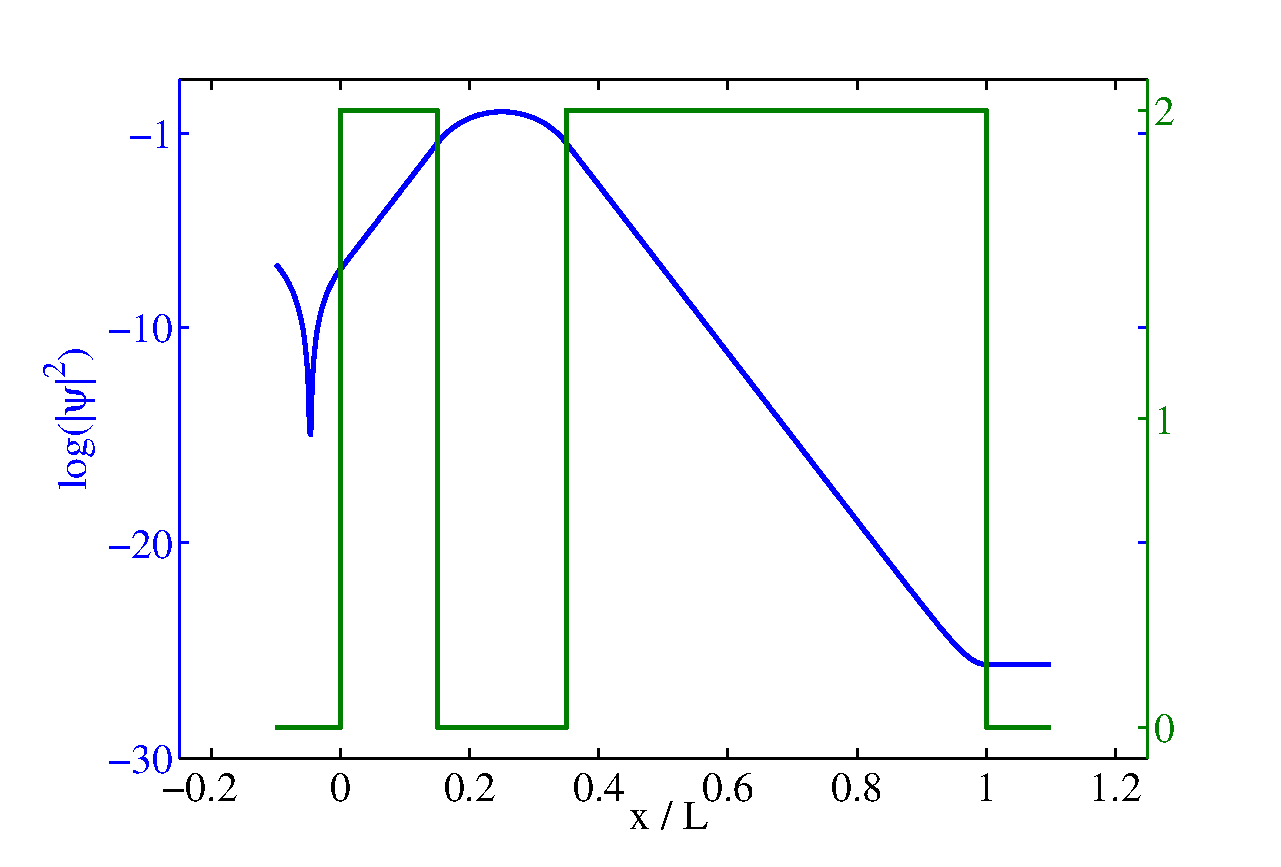
\includegraphics{pictures/barrier_defect_at_14_waveform_log}}
\scalebox{0.3}{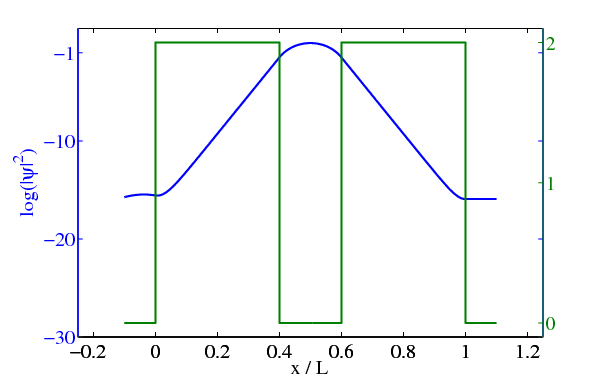
\includegraphics{pictures/barrier_defect_at_12_waveform_log}}
\scalebox{0.3}{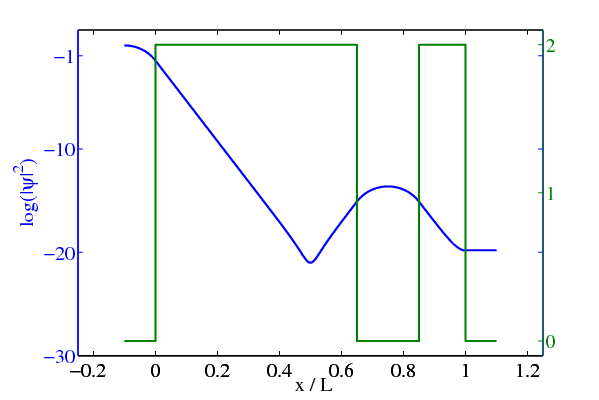
\includegraphics{pictures/barrier_defect_at_34_waveform_log}}}
\vskip -0.5cm
\caption[A wave incident from the left (solid blue line) on a potential barrier with potential well (dotted green) on semilogy scale looks  very similar to the electric field (aka energy) in the random system (Fig.~\ref{fig:peaksmatchnotmatch}).]{A wave incident from the left (solid blue line) on a potential barrier with potential well (dotted green) on semilogy scale looks  very similar to the electric field (aka energy) in the random system (Fig.~\ref{fig:peaksmatchnotmatch}).
We hypothosize that tunneling may be the reason for the
exponential decay and growth. Also seen in 
\cite{2004_Bliokh_wavelet}, but this is cleaner.}
\label{fig:barrierdefectlog}
\end{figure}

In the periodic layers with single defect the plots are the similar to the potential barrier model results, but with a more pronounced peak. For this analytical model we manually position the defect (instead of the potential well).

\begin{comment}
\begin{figure}
\vskip -0.5cm
\centerline{
\scalebox{0.3}{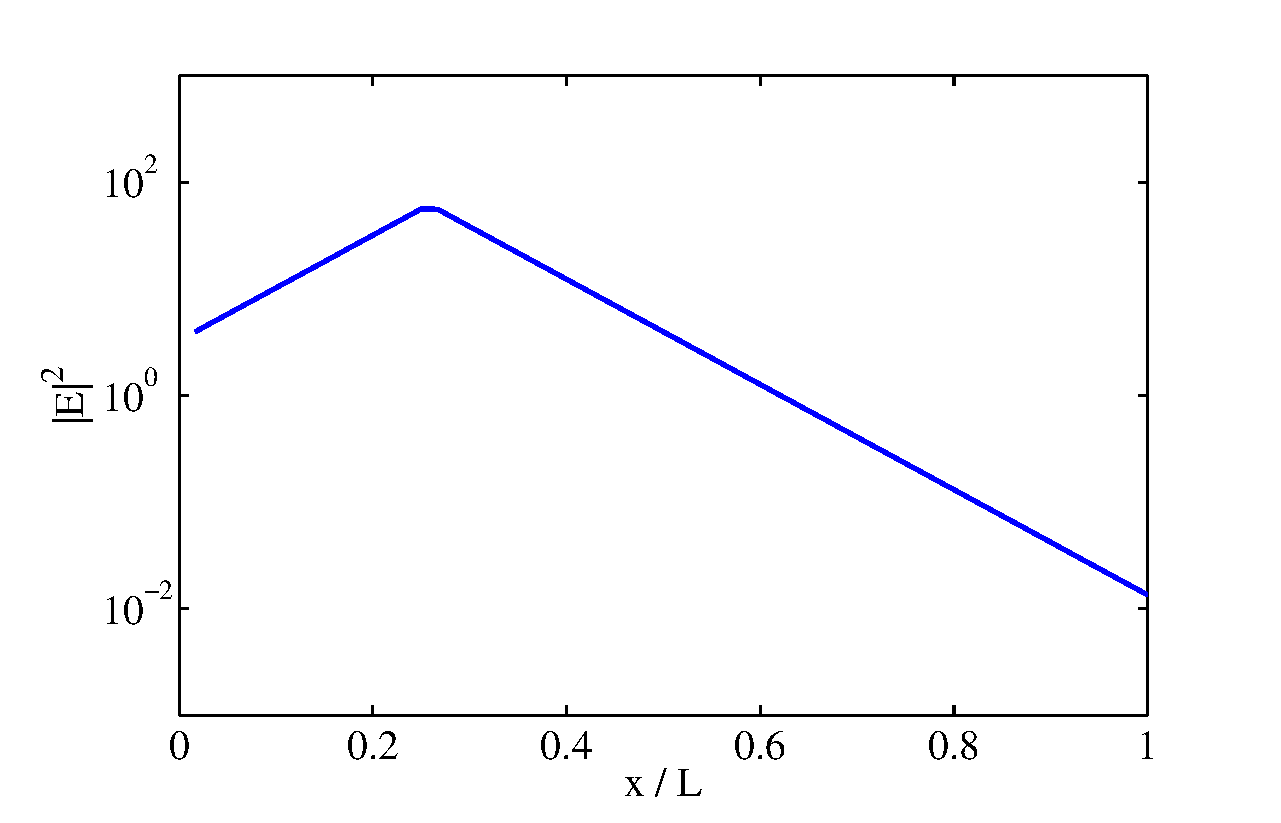
\includegraphics{pictures/passive_defect_14}}
\scalebox{0.3}{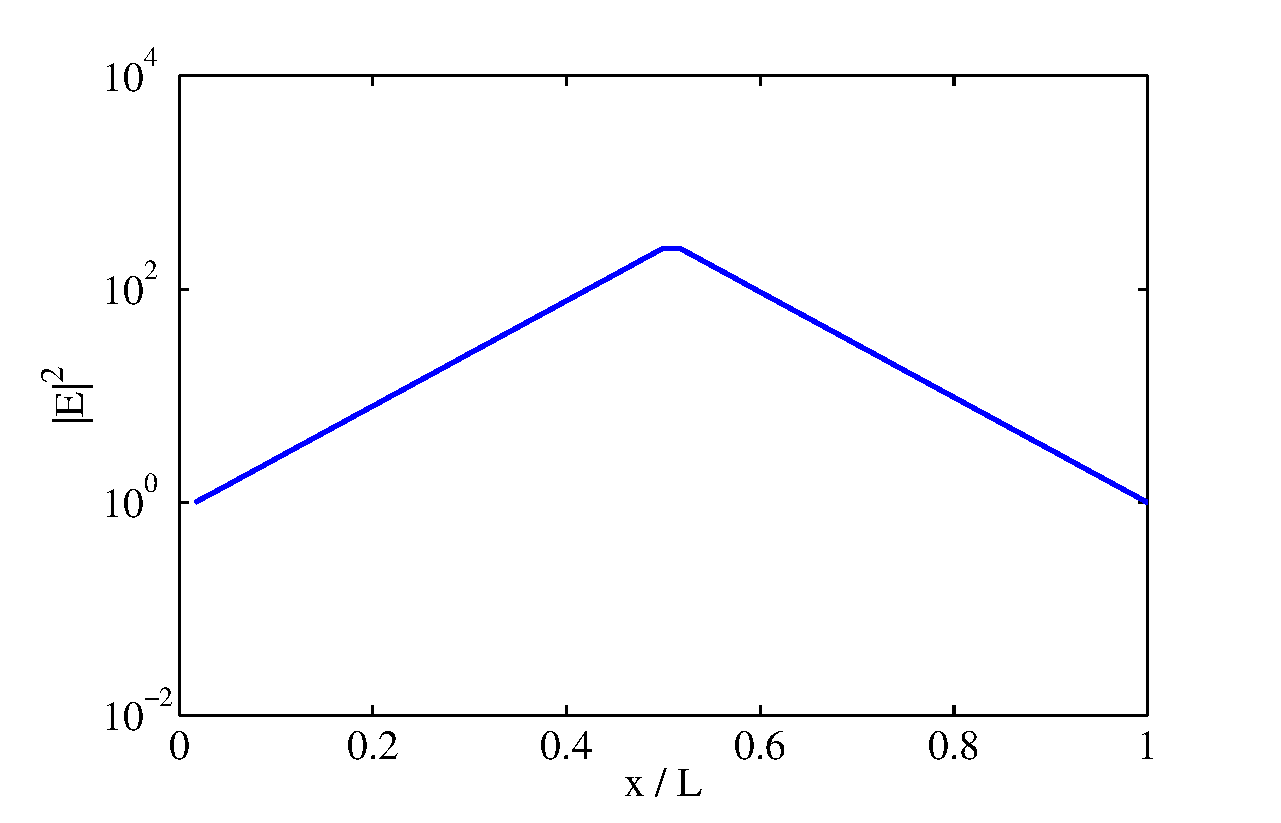
\includegraphics{pictures/passive_defect_12}}
\scalebox{0.3}{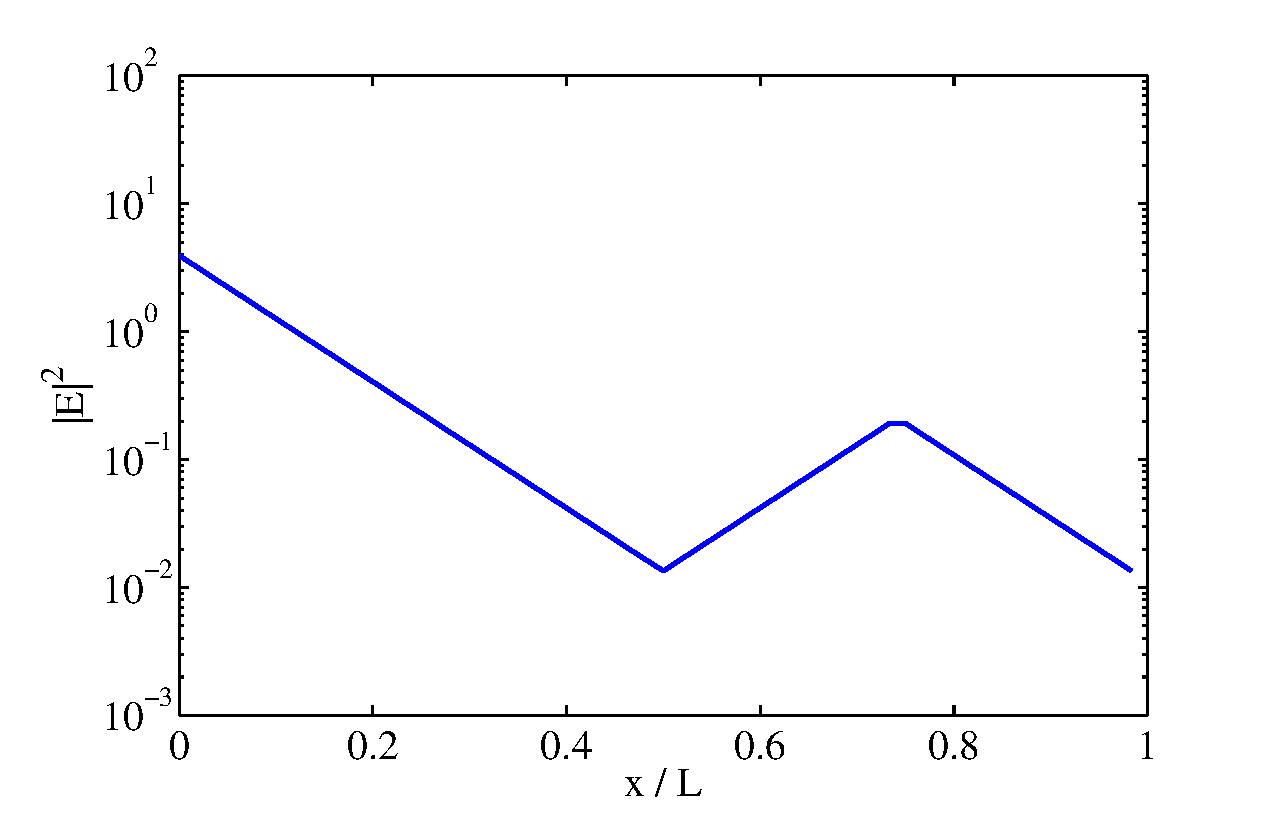
\includegraphics{pictures/passive_defect_34}}}
\vskip -0.5cm
\caption[The three plots correspond to a single defect at at $\frac{1}{4}$L, $\frac{1}{2}$L, and $\frac{3}{4}$L, respectively, for the passive periodic system
on semilogy scale (another analytical model).]{The three plots correspond to a single defect at at $\frac{1}{4}$L, $\frac{1}{2}$L, and $\frac{3}{4}$L, respectively, for the passive periodic system
on semilogy scale (another analytical model). We see the same
results we saw for Fig.~\ref{fig:barrierdefectlog} so
now we are confident that tunneling is causing the effect
seen in Fig.~\ref{fig:peaksmatchnotmatch}.}
%\label{fig:passivedefect}
\end{figure}
\end{comment}

These three models (random dielectric layers, potential barrier, and periodic layers) are closely related since all three are wave based.

Based on the passive analytical models we gain confidence that the light is tunneling through the material.  If there is a center of localization present in the random layers this is akin to the light tunneling to the potential well between the barriers and then tunneling out.

Also based on the analytical models we determine that the position of the center of localization/potential well/single defect directly affects how much energy is stored in the system.

\begin{comment}
\begin{figure}
\vskip -0.5cm
\centerline{
\scalebox{0.5}{\includegraphics{pictures/T_E_on_resonance_vs_xo}}}
\vskip -0.5cm
\caption[Transmission and energy and their ratio as a function of
the position of the center of localization.]{Transmission and energy and their ratio as a function of
the position of the center of localization. The energy plot is
similar to the theoretical energy in Fig.~\ref{fig:peaksmatchnotmatch}
As a result of the asymmetry in energy with respect
to defect position, the ratio of transmission to energy is not constant.}
\label{fig:defectpositionTE}
\end{figure}
\end{comment}

This variation of stored energy based on the position of
the center of localization explains why there are peaks
in energy but not always corresponding peaks in energy.
It also explains why peaks in energy imply peaks 
in transmission: the energy stored in the sample
means there is a center of localization in the sample, which
allows for increased transmission.  Now when we see a transmission and
energy plot versus frequency we can determine the location
of the center of localization by inspection.  If there is
a peak in transmission and energy,
then $ 0 < x < \frac{1}{2} L $.  If there is a peak
in transmission but not energy then the center of
localization is between $ \frac{1}{2} L < x < L $.

Presence of a center of localization for some frequency can be detected
through the deviations from a simple exponential 
decay in the field distribution inside the sample.

%%%%%%%%%%%%%%%%%%%%%%%%%%%%%%%%%%%%%%%%%%%%%%%%%%%%%%%%%
\subsubsection {Theory of Passive 1-D Systems}
%%%%%%%%%%%%%%%%%%%%%%%%%%%%%%%%%%%%%%%%%%%%%%%%%%%%%%%%%

% warning: the following figure may be redundant
% it is included for initial conceptual understanding

\begin{figure}
\vskip -0.5cm
\centerline{
\scalebox{0.9}{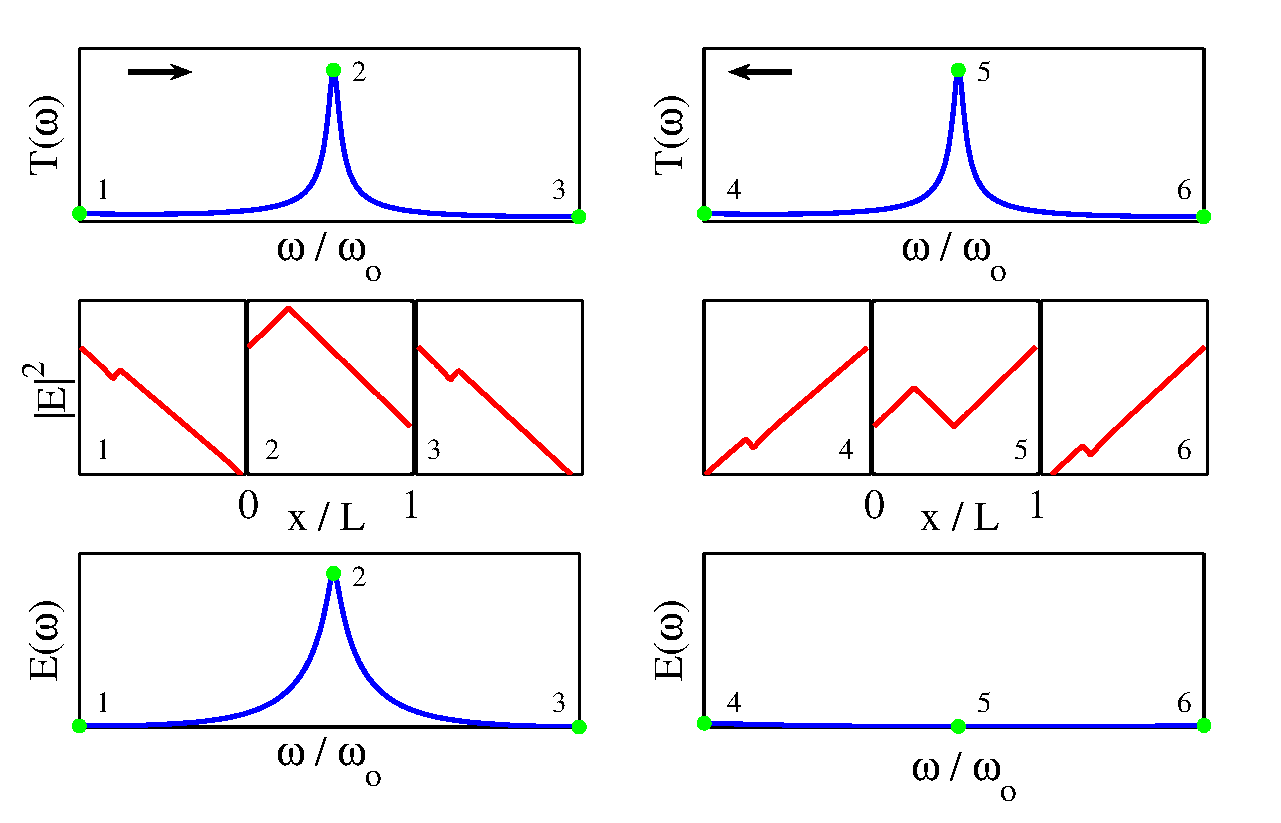
\includegraphics{pictures/peaks_match_peaks_dont_match}}}
\vskip -0.5cm
\caption[The above plots are from the periodic layers with
single defect model.]{The above plots are from the periodic layers with
single defect model. The left half are from the defect occuring
at $ \frac{1}{4} $L and the right set of plots are from the defect
at $ \frac{3}{4} $L, all without gain.  The top plot on both 
sides is transmission versus frequency centered at the resonant
frequency. For both $ \frac{1}{4} $L and $ \frac{3}{4} $L the resonant
frequency means a spike in transmission.  However, the lower plot
on both side (Energy versus frequency) shows that the amount of
energy is dependent on the defect position (which corresponds to
the center of localization in a random model).  Looking at
the behavior of the energy inside the sample for resonant
and off-resonant frequencies, the behavior of the wave changes
as close the resonant frequency. When off resonance there is
pure exponential decay, which translates to a straight decreasing
slope on the semilogy scale. On resonance there is a peak in energy
for both defect positions. However, the total energy in the sample
is much less for $ \frac{3}{4} $L (remember that these are semilogy
plots).  This demonstrates why T/${\cal E}$ is not constant in passive samples:
the ratio is affected by the position of the defect (center of localization
for random layers).}
%In the upper left figure we suppose there is 
%a peak in energy and corresponding peak in transmission.
%The amount of  energy in the sample is relatively large.
%In the upper right sketch we see what happens when 
%there is no peak in energy but there is a peak in transmission:
%much less energy is in the sample. 
%When the amount of energy in the media is plotted 
%as a function of center of localization, we see that there is an asymmetry.
%This is why T/${\cal E}$ is not smooth - it ratio is affected 
%by the position of the center of localization.}
\label{fig:peaksmatchnotmatch}
\end{figure}

We derive the T/${\cal E}$ ratio. The transmission T as a 
function of frequency $\omega$ and center of localization position $x_o$ 
is a lorentz distribution of the form

\begin{equation}
T = T(\omega, x_o) = \frac{(\exp(-\frac{L}{\xi}))^2}{ 
(\omega-\omega _o)^2 + (\exp(-\frac{L}{\xi})\frac{1}{2}\exp(\frac{\mid L-2 x_o \mid}{\xi}))^2 }
\label{eq:transmission}
\end{equation}
Where we have appoximated cosh() as $\frac{1}{2}\exp()$. 


From work done in Appendix B,
\begin{equation}
{\cal E}(x,\omega) = \frac{\xi}{2} ( T ( \exp\left(\frac{2(L-x_o)}{\xi}\right) - \exp\left(\frac{2(L-2 x_o+x_1)}{\xi}\right) + \exp\left(\frac{2(L-x_o))}{\xi}\right) -1 ) + 4 (1-\exp\left(-\frac{2 x_1}{\xi}\right)) )
\label{fig:energy}
\end{equation}

As a check on Energy we can look at the resonant frequencies as the center of localization position $x_o$ varies. We recover Fig.~\ref{fig:energydistrib}.

\begin{figure}
\vskip -0.5cm
\centerline{
\scalebox{0.5}{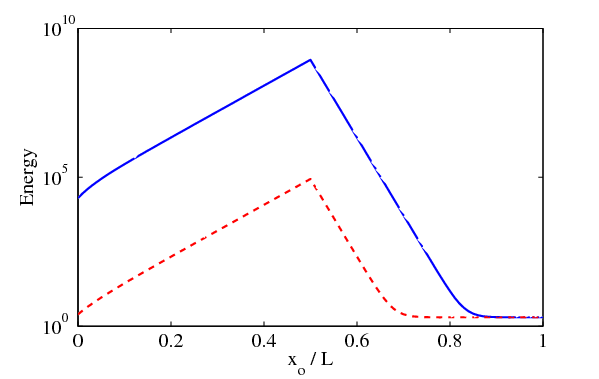
\includegraphics{pictures/energy_distribution_g0_and_99gc}}}
\vskip -0.5cm
\caption{Energy distribution as a function of position of center
of localization $x_0$ on resonant frequencies without gain (dotted
red) and with 99\% of critical gain (upper solid blue). See 
Eq.~\ref{fig:energy}. These
plots show why the peaks in transmission do not always have a corresponding
peak in energy, as seen in Fig.~\ref{fig:peaksmatchnotmatch}. and 
Fig.~\ref{fig:tenkenergytransmission}. Even when gain is added the 
asymmetry does not go away.}
\label{fig:energydistrib}
\end{figure}

Now we will look only at resonant frequencies
($\omega = \omega_0$) with sufficient gain that $x_1$ goes to zero (then
$y_2$ has a range from zero to $x_1$. This includes passive systems where the defect is in
the first half of the sample and if the defect is in
the second half, then the gain is sufficient that there 
is no initial exponential decay regardless of defect position. Visually, the plot has a single clusp.  

\begin{equation}
\frac{\cal E}{T} = \frac{\xi}{2} ( 2 \exp\left(\frac{2(L-x_0)}{\xi}\right) - \exp\left(\frac{2(L-2 x_0)}{\xi}\right) -1 ) )
\end{equation}

\begin{figure}
\vskip -0.5cm
\centerline{
\scalebox{0.5}{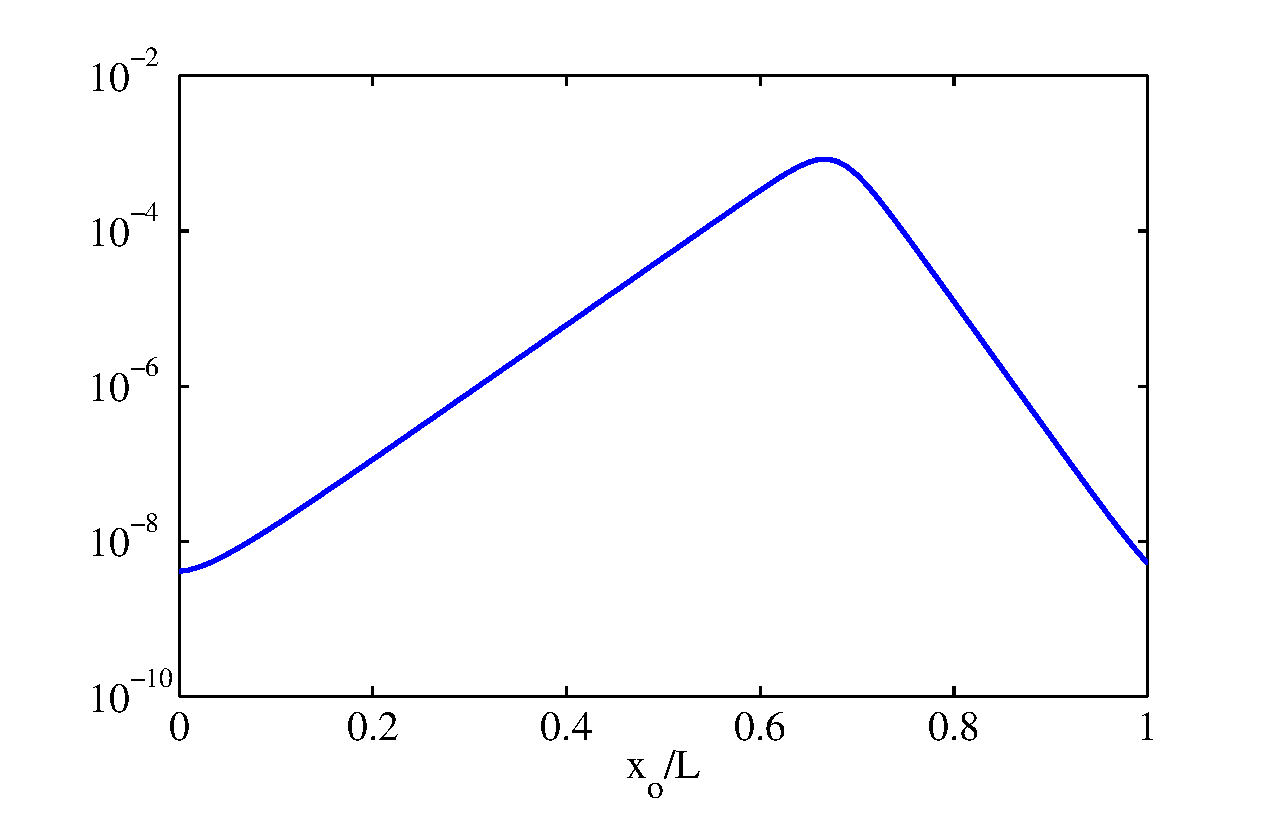
\includegraphics{pictures/log_TE_v_defect_position_passive}}}
\vskip -0.5cm
\caption{Transmission/Energy as a function of position of center
of localization $x_0$ on resonant frequencies without gain. Eq.~\ref{fig:energy}
divided by Eq.~\ref{fig:correctedtransmission}. This is why T/${\cal E}$ will not work
for a criteria; the ratio depends on where the center of localization occurs. 
One can not average over all possible positions.}
\label{fig:energytranspassive}
\end{figure}

If we assume $x_0$ is not near the edges of the sample $x_0 > 0$ and $x_0 < L$ with $L > \xi$ then we can drop the last two terms, leaving
\begin{equation}
\frac{\cal E}{T} = \xi \exp\left(\frac{2(L-x_0)}{\xi}\right)
\end{equation}

Inverting that to get T/${\cal E}$,

\begin{equation}
\frac{T}{\cal E} = \frac{1}{\xi} \exp\left(-\frac{2(L-x_o)}{\xi}\right)
\end{equation}

Note that the log of either results in a non-exponential form which could be integrated. Neither T/${\cal E}$ nor ${\cal E}$/T is particularly useful. When one averages ${\cal E}$/T the background dominates, whereas for T/${\cal E}$ the resonant frequency behavior dominates. See Fig.~\ref{fig:logTEET}.

\begin{figure}
\vskip -0.5cm
\centerline{
\scalebox{0.5}{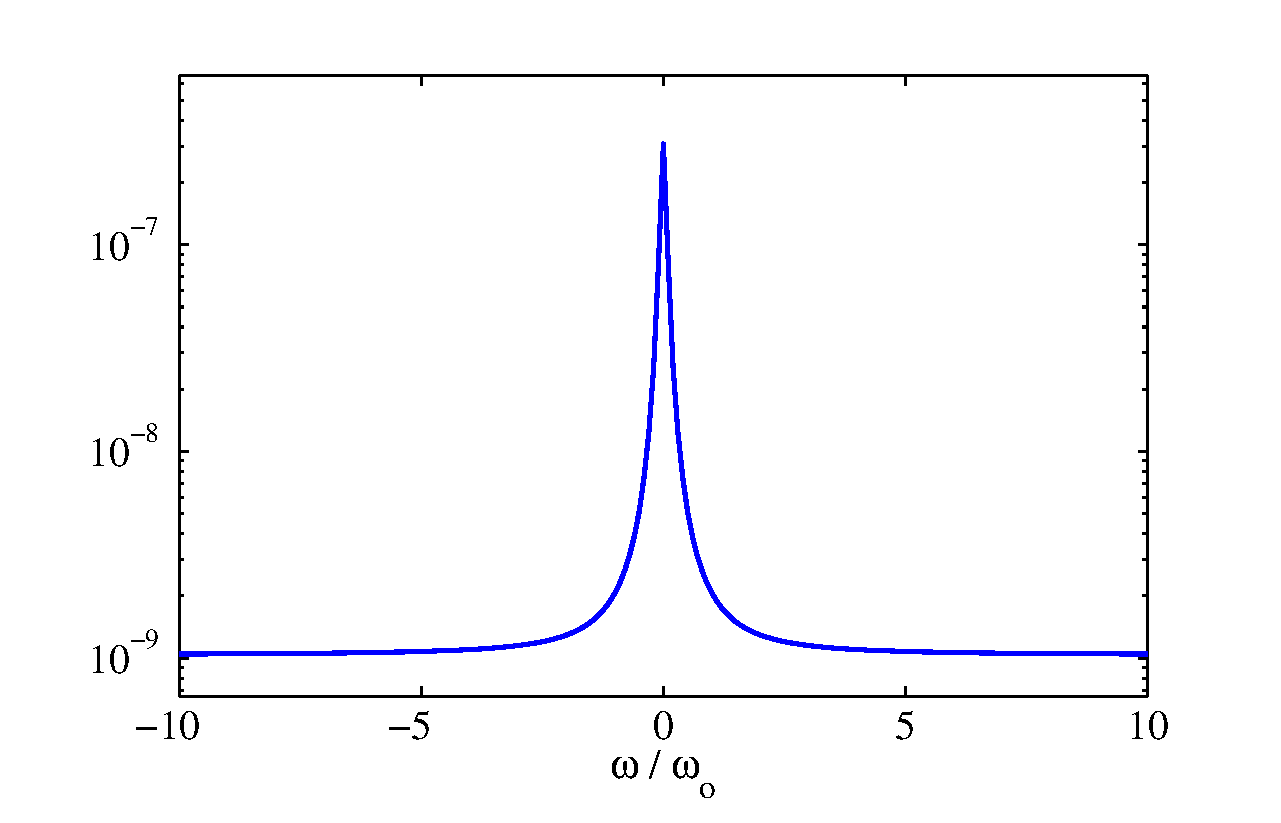
\includegraphics{pictures/log_TE_v_freq}}}
\vskip -0.5cm
\caption{T/${\cal E}$ versus frequency for passive systems
with the correction from Eq.~\ref{fig:correctedtransmission}. Frequency 
is zero on resonance. This plot show that
if T/${\cal E}$ is attempted to be used as a criteria for 
finding localization for an ensemble of samples, the peak and background
obsure each other. The problem is the same for ${\cal E}$/T.}
\label{fig:logTEET}
\end{figure}

When gain is added, the left boundary condition ($y_1=4$ at $x=0$) is no
longer valid. The entire field distribution grows in height, including
the end points. This would be equivalent to letting $x_1$ (the turning
point) become negative, which is non-physical. In order to prevent this
we change the limits of integration to be max($x_1$,0) instead of $x_1$ 
in Eq.~\ref{fig:Eintegral}.

Another problem arises with T from Eq.~\ref{eq:transmission} in 
that the ``worst case'' (minimum for T) is when we are so far off resonance
that only exponential decay occurs. As the above equations are given
T goes to zero, which is incorrect. Physically, T asymptotically reaches the exponential
decay value. Thus in order to make this correction, we shift the 
Eq.~\ref{fig:transmission} up by the exponential decay background.

\begin{equation}
T = T(\omega, x_0) = \frac{(\exp(-\frac{L}{\xi}))^2}{
(\omega-\omega _0)^2 + (\exp(-\frac{L}{\xi})\frac{1}{2}\exp(\frac{\mid L-2 x_0 \mid}{\xi})-g)^2
} + \exp\left(-\frac{L}{\xi}\right)^2
\label{fig:correctedtransmission}
\end{equation}

%%%%%%%%%%%%%%%%%%%%%%%%%%%%%%%%%%%%%%%%%%%%%%%%%%%%%%%%%
\subsubsection {Adding Gain}
%%%%%%%%%%%%%%%%%%%%%%%%%%%%%%%%%%%%%%%%%%%%%%%%%%%%%%%%%

Now we understand why the ratio of transmission to energy (T/${\cal E}$) is not smooth in passive systems: the ratio depends on the position of the center of localization. When gain is added to the random system we hope that T/${\cal E}$ becomes smoother because we do not expect such a dramatic dependence on the position of the localization center.

In order to reach the critical gain we investigate the periodic system with single defect. We did not test the addition of gain in the double potential single well model.

When gain is added to the three canonical cases we see a rise in the peaks and the peak position remains the same. The tail for the $ \frac{3}{4} $L does not change, only the peak increases.  (Fig.~\ref{fig:periodicdefect}).

\begin{figure}
\vskip -0.5cm
\centerline{
\scalebox{0.3}{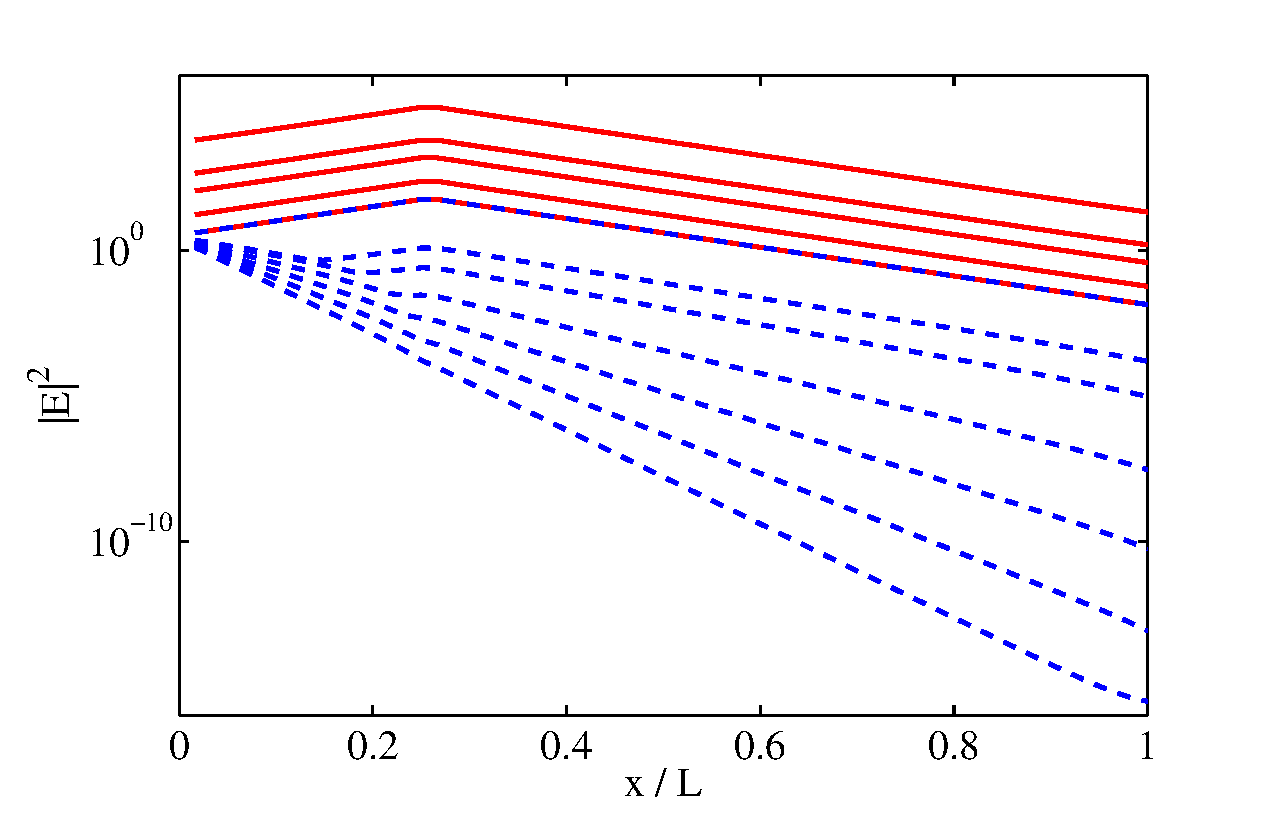
\includegraphics{pictures/periodic_14_defect_absorb_to_gain}}
\scalebox{0.3}{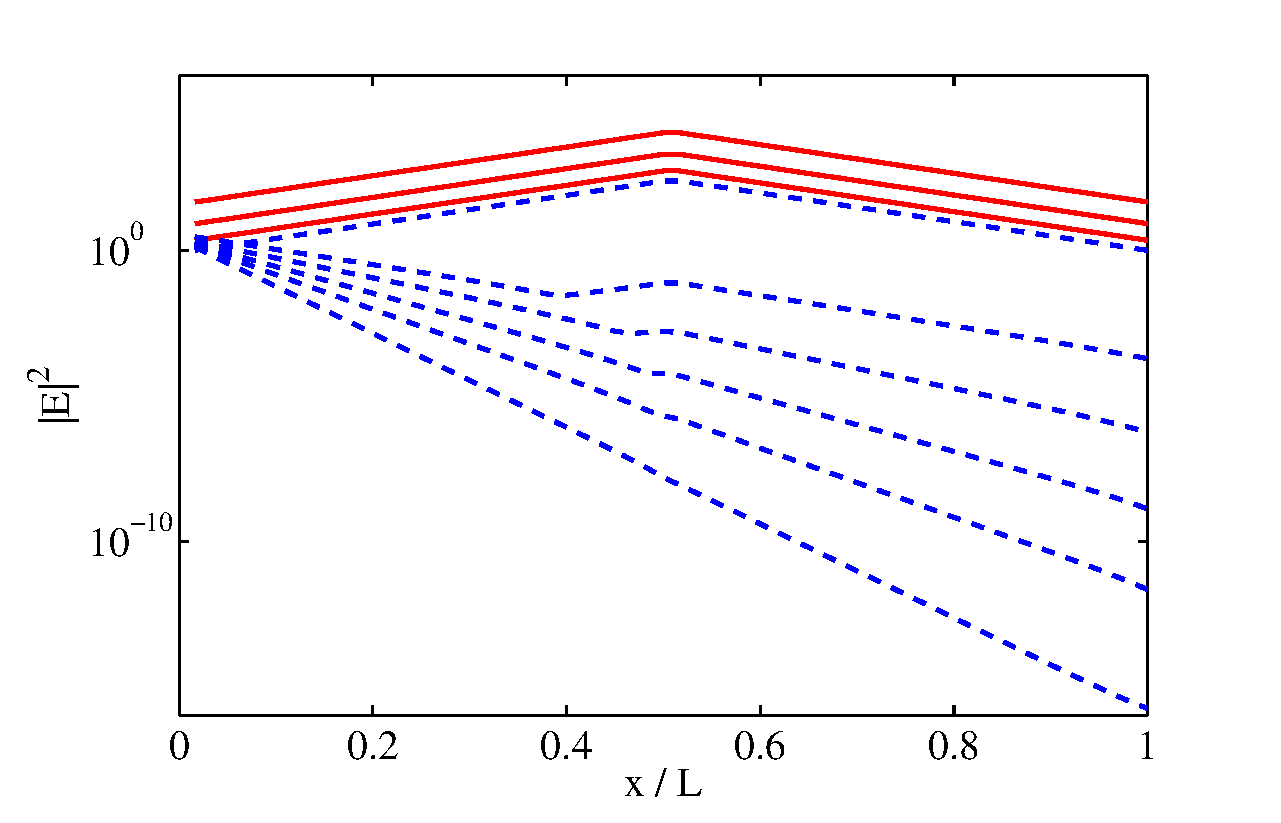
\includegraphics{pictures/periodic_12_defect_absorb_to_gain}}
\scalebox{0.3}{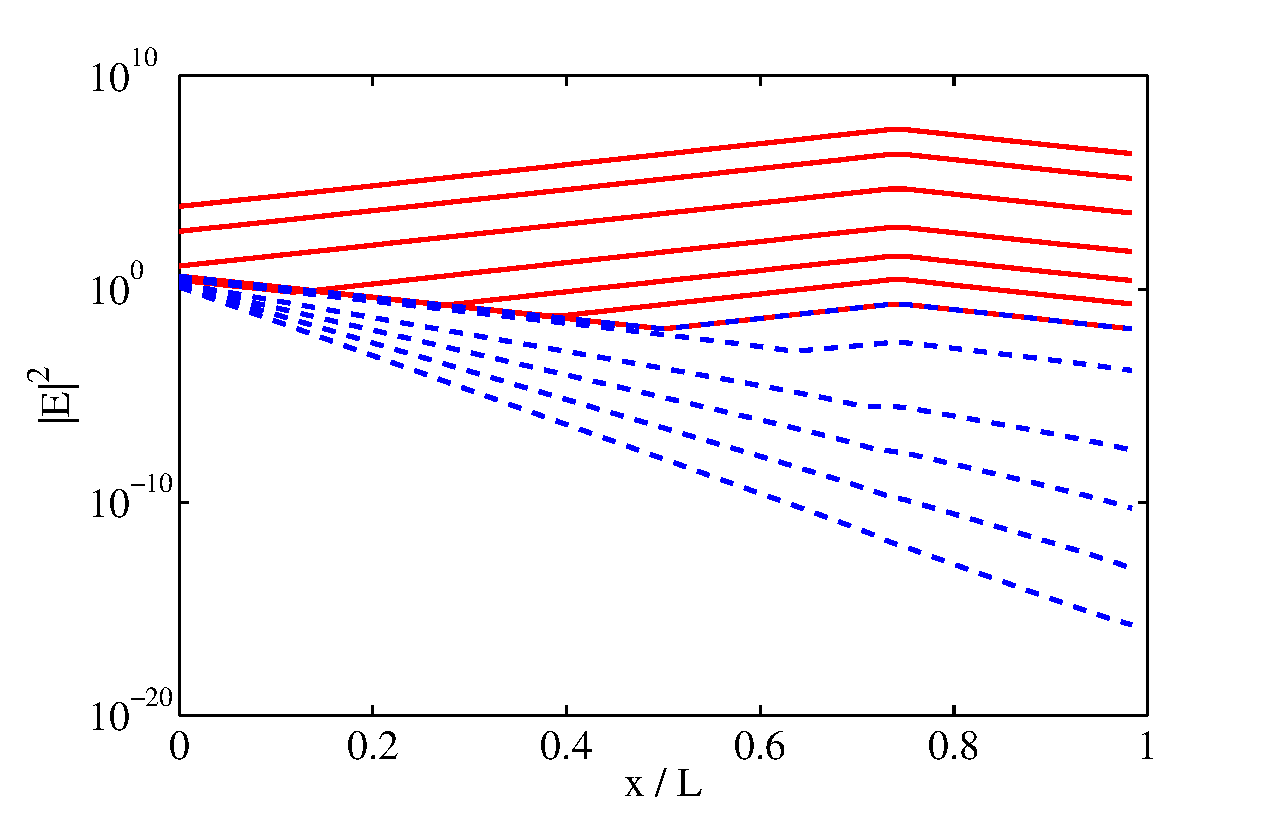
\includegraphics{pictures/periodic_34_defect_absorb_to_gain}}}
\vskip -0.5cm
\caption[The log of the field in the sample for three canonical positions for the periodic 1-D structure with single defect.]{The log of the field in the sample for three canonical positions for the periodic 1-D structure with single defect. In this analytical model the single anomalous layer is at $ \frac{1}{4} $L, $ \frac{1}{2} $L, and $ \frac{3}{4} $L, respectively and the amount of absorption or gain is varied. The lowest dotted blue straight line is full absorption. On a log scale the exponential scale appears as a more obvious straight negative slope line. As absorption is decreased and the passive system is approached a turning point appears. For the $ \frac{1}{4} $L and $ \frac{1}{2} $L systems this turning point disappears at the passive system incident side. Then gain is added to the model (solid red line). For the $ \frac{1}{4} $L and $ \frac{1}{2} $L defects the peak simply increases, as expected in active media. For the $ \frac{3}{4} $L system the turning point moves toward the incident side. Thus in active media the wave form changes for defects occuring in the second half of the sample. Eventually the gain is sufficient that the $ \frac{3}{4} $L position is symmetric with the  $ \frac{1}{2} $L position. Now in all three canonical positions with gain the field in the sample grows exponentially to a peak before falling.}
%The analytical periodic model with defects at . We scan from the absorption (blue) regime
%to gain (red).}
\label{fig:periodicdefect}
\end{figure}

Note that near the critical gain, the transmission and the field distribution inside the sample becomes very sensitive to the amount of gain added to the system. %[foreshadowing.]

At the critical gain the defect at $ \frac{1}{4} $L and the
defect at $ \frac{3}{4} $L
cases are symmetric with respect to each other about the y axis.
The defect at $ \frac{1}{2} $L is symmetric about x=$ \frac{1}{2} $L
and the defect at $ \frac{1}{4} $L would be symmetric
with the defect at $ \frac{3}{4} $L if
it were flipped around. [Foreshadowing, we will get back to this.]

At the critical gain the ratio of transmission to energy
is smoother than the passive system,
but there are some issues for when the center of
localization is between $ \frac{1}{2}$L and L. We have
found that T/${\cal E}$ is
a ``good'' parameter for 1-D systems with gain, in that it is
not divergent (unlike T and ${\cal E}$ are separately).  It can be
measurable.  However, it is not perfect as it depends on sample orientation.

%%%%%%%%%%%%%%%%%%%%%%%%%%%%%%%%%%%%%%%%%%%%%%%%%%%%%%%%%
\subsubsection {Closed and Open Systems Theory for Passive 1D Models}
%{closed and open systems: the importance of phase}
%%%%%%%%%%%%%%%%%%%%%%%%%%%%%%%%%%%%%%%%%%%%%%%%%%%%%%%%%

The idea of flipping the sample orientation warrants
attention.  If there is a center of localization
at $ \frac{1}{4} $L and
the sample is flipped (sample goes from L to 0 instead
of the standard 0 to L) then we know there will be a center
of localization at $ \frac{3}{4} $L.  The waveform for
these two localization centers is the same in the region
of localization.

An equivalent to flipping the sample orientation is
to change the orientation of the light.  If one keeps
the sample fixed and shines light on the x=L side of the
sample then we get the same result as fixing the light and
flipping the sample orientation.  The math is slightly
different for the two cases. %As flipping the light source
%is more common in literature we will stick with that.

We will call the case where light is incident on the left side ``LR''
as light moves left to right. Conversely we will call the
light being incident on the right side ``RL''.  Also,
we will call the resulting LR field 
distribution $ \psi _1(x) $ and the RL wave $ \psi  _2(x) $. 
The flipping we will term ``reciprocity.'' 

A reality check for flipping the sample (or flipping the
light source) is that the transmission should be the same for the
two cases since the light is traveling through the
same material.  Note that flipping both the sample and the
light gets one back to the original setup.

Thouless criteria says that a small change in boundary
conditions should not affect energy spectrum. However, we 
find that flipping the beam (which is a small change
in boundary conditions) does cause an enormous 
change {\it in the waveform in the sample}. This  affects
how much energy is in the system, ie the waveform for
localization at $ \frac{1}{4} $L becomes the
waveform for localization at $ \frac{3}{4} $L.
There is a lot less energy in the system for the
$ \frac{3}{4} $L waveform as compared to $ \frac{1}{4} $L. A
small change in the boundary conditions leads to
a significant change in how much energy is stored
in the sample.

How can reciprocity help to identify localization? Experimentally one can shine light on either side of a given sample, so reciprocity is straight forward to execute.  What follows is	% don't tell experimentalist what is "easy"
the mathematical analysis of using reciprocity.

We start by showing that the two wave forms are functionally independent by finding the Wronskain for the left sides of the two orientations. It can be shown that for our Maxwell equation the Wronskian is position independent.
 % see notes 20080117

\begin{figure}
\vskip -0.5cm
\centerline{
\scalebox{0.8}{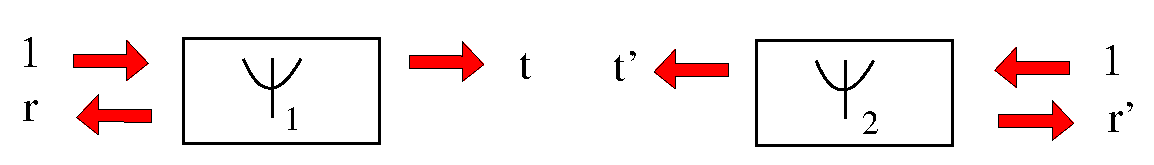
\includegraphics{pictures/wronskian_LR_RL}}}
\vskip -0.5cm
\caption[For the two orientations, left-to-right and right-to-left, two wave functions are assigned: $ \psi _1$ and $ \psi _2$.]{For the two orientations, left-to-right and right-to-left, two wave functions are assigned: $ \psi _1$ and $ \psi _2$. The wronskian for is the same for both since the transmission is the same for both orientations.}
\label{fig:wronskainLRRL}
\end{figure}

\begin{equation}
\begin{vmatrix}
1 \exp(i k x) + r \exp(-i k x) & t' \exp(-i k x) \\
i k \exp(i k x) - i k r \exp(-i k x) & i k t' \exp(i k x)
\end{vmatrix}
 = -2 i k t'
\label{eq:wronskleft}
\end{equation}

Similarly, the Wronskain for the right sides is: % semi-redundant

\begin{equation}
\begin{vmatrix}
 t \exp(i k x) & 1 \exp(-i k x) + r' \exp(i k x)\\
i k t \exp(i k x) & -i k \exp(-i k x) + i k r' \exp(-i k x)
\end{vmatrix}
 = -2 i k t
 \label{eq:wronskright}
\end{equation}

Note that the two Wronskians are non-zero and are the same since t = t'. Now that we have to independent functions we can use them as a basis to create a new linear combination.

An analog is the one dimensional potential well with an eigen state in the well.In a closed system we can find eigen states and eigen frequencies.  For the passive random model this would be equivalent to adding mirrors to the edges of the sample so that no light escapes to the environment.

For the open system (both for potentials and in the case we are working with, layers of dielectric) there will be two solutions, a left and right traveling wave.  For closed systems there is one solution (composed of two waves - standing wave).

Closed system solution can be expressed in terms of $\psi _1(x), \psi _2(x)$:
\begin{equation}
\psi (x) = c_1  \psi _1(x) + c_2  \psi _2(x)
\end{equation}
%   Y(x) = c_1 Y_1(x) + c_2 Y_2(x)
where $\psi _1$ and $ \psi  _2 $ are the wave functions associated with the LR and RL orientations in the random system. To find the eigenstates apply the boundary conditions: the function $\psi$(x) is zero at the edges of the closed system. 
\begin{equation}
\begin{gathered}
\psi (x=0) = c_1  \psi _1(0) + c_2  \psi _2(0) = 0 \\
\psi (x=L) = c_1  \psi _1(L) + c_2  \psi _2(L) = 0
\end{gathered}
\end{equation}
%  Y(0) = c_1 Y_1(0) + c_2 Y_2(0) = 0
%  Y(L) = c_1 Y_1(L) + c_2 Y_2(L) = 0
This can only be valid when the determinant is zero
\begin{equation}
det
\begin{bmatrix}
\psi _1(0) & \psi _2(0) \\
\psi ' _1(L) & \psi ' _2(L) 
\end{bmatrix}
 = 0
\end{equation}

This $ \psi _1 $ and $ \psi _2 $ can be interpreted as either the electric field at the edges or related to the reflection and transmission coefficients:
\begin{equation} % see notes 20080130
\begin{gathered}
E(0) =  \psi _1 (0) = 1+r \\
k E'(0) = \psi ' _1 (0) = k i (1-r)
\end{gathered}
\end{equation}
or equivalently t t' - (1+r) (1+r') = 0. %notes 20080117 last page

Now we can go back to the random system and find the determinant given $\psi  _1$(x) and $\psi _2 $(x). When the determinant is zero that implies the frequency is an eigen frequency (in a closed system) and the wave function is an eigenstate.  Since the layers actually make an open system, we will call these ``resonant frequencies.'' Scanning the range of frequencies yields points on the T and ${\cal E}$ versus frequency plot that correspond (perfectly) with the peaks in energy in transmission.

Note that when the transmission and energy versus frequency is plotted then the transmission for the LR and RL cases is the same (t=t'), whereas the energy is not the same for the LR and RL orientation. The energy peaks at different frequencies, resulting in two lines for energy, whereas there is one for transmission.  The dots are where the determinant is zero.

\begin{figure}
\vskip -0.5cm
\centerline{
\scalebox{0.5}{\includegraphics{pictures/trans_energy_det}}} 
\vskip -0.5cm
\caption[Transmission, energy, and determinant=0 for LR and RL orientations versus frequency.]{Transmission, energy, and determinant=0 for LR and RL orientations versus frequency. This is similar to Fig.~\ref{fig:tenkenergytransmission}, except now we can predict where the peaks occur.}
\label{fig:energytransmissiondet}
\end{figure}
We can test that the states at these resonant frequencies are orthogonal. See Deych's paper\cite{2005_Deych}.
% see notes 20080214
\begin{equation}
\frac{\int _0 ^L \psi _1 \psi _2 ^* \epsilon(x) dx}
{\sqrt{\int _0 ^L \psi _1 \psi _1 ^* \epsilon(x) dx}
 \sqrt{\int _0 ^L \psi _2 \psi _2 ^* \epsilon(x) dx}} = 0
\end{equation}

%20080213 page 1
Note that when the center of localization is at $ \frac{1}{4} $L for resonant frequencies the electric field at x=0 is close to zero.  (See Fig.~\ref{fig:standingwave}.) Reason: the waves outside the material are cancelling out due to interference.  This results in a standing wave.   r=-1 (from 1+r=0).

\begin{figure}
\vskip -0.5cm
\centerline{
   \scalebox{0.5}{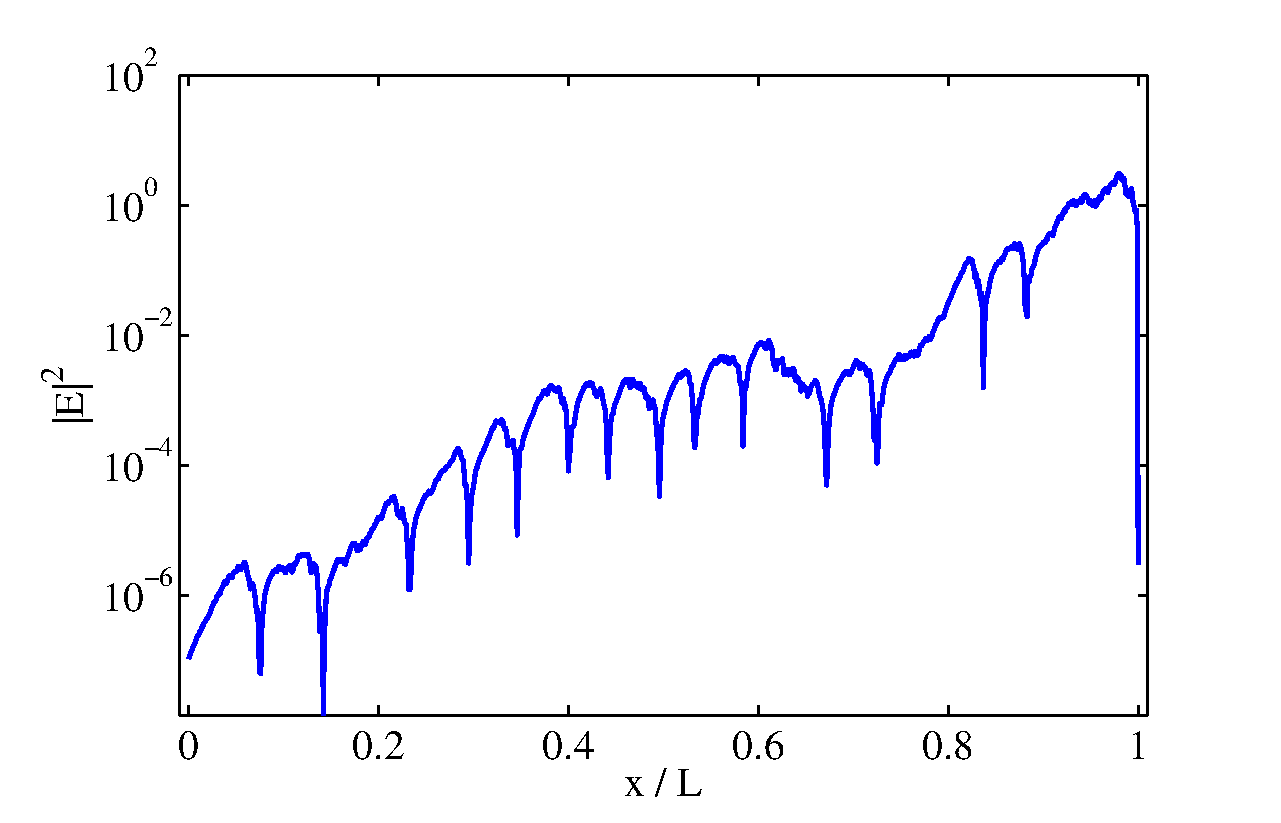
\includegraphics{pictures/standing_wave_electric_field}}
}
\vskip -0.5cm
\caption[A resonant frequency showing drop-off at x=L.]{A resonant frequency showing drop-off at x=L. Even though the center of localization may not be obvious for this resonant frequency, the fact that the electric field approaches zero on both sides of the sample means the field is approaching a closed system resonance.}
\label{fig:standingwave}
\end{figure}

This is a reliable and accurate method for find lasing threshold in computational models. To find the critical gain first find a resonant frequency by calculating where the determinant is zero. Then for each resonant frequency plot the transmission versus gain. The transmission will diverge at critical gain. The amount of gain added becomes very sensitive near the critical gain, but one can find arbitrarily small bounds on what the critical gain is by zooming in on the peak.

An alternative method for finding the critical gain is to look at the transmission versus frequency plot and measure the full width at half maximum (FWHM), $\gamma$.
\begin{equation}
g_{critical} = \frac{\gamma}{2} / \frac{2 \pi}{ \lambda }
% old: \frac{\frac{\gamma}{2}}  {\frac{2 \pi}{ \lambda }}
\end{equation}

Experimentally the light has to be shone from both left-to-right and right-to-left, but the result is to find what would be eigen frequencies of the closed system.  We will still call these the resonant frequencies since we are in the open system.

As a reality check, the wave coefficients A and B should be equal throughout the sample at resonant frequencies since the left and right-traveling waves are equal (see Fig.~\ref{fig:ABLRRLlog}.  A=B also implies that there is no oscillation in energy at the resonant frequency, thus there is no energy leakage out of the sample.

If A=B then the two complex waves should sum to a real wave:
\begin{equation}
A \exp(i k x)+A \exp(-i k x) = A \cos(k x)
\end{equation}

\begin{figure}
\vskip -0.5cm
\centerline{\scalebox{0.8}{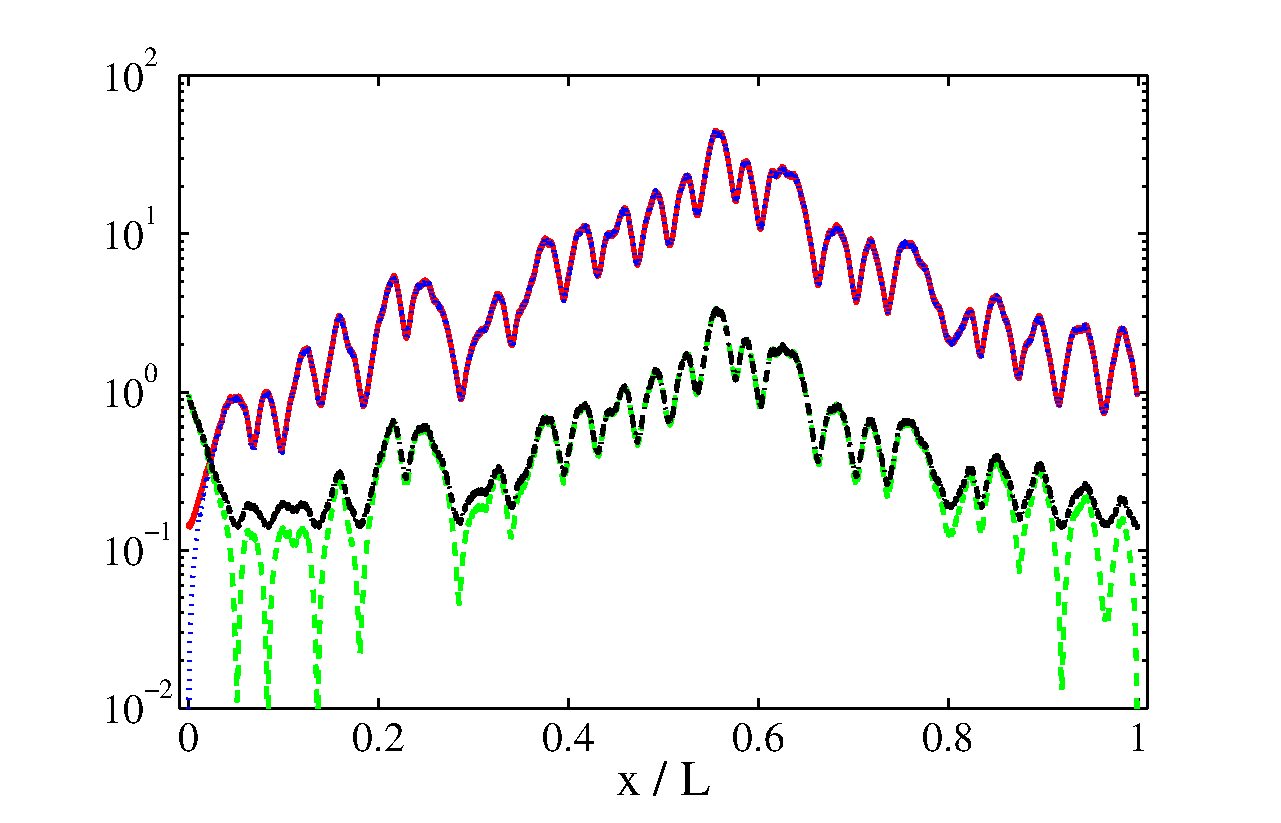
\includegraphics{pictures/AB_LR_and_RL}}}
\vskip -0.5cm
\caption[A and B coefficients for the two orientations (left to right and right to left).]{A and B coefficients for the two orientations (left to right and right to left). The lower two lines (dotted green and dotted black) are the backward (B) and forward (A) propagation coeffients, respectively of the electric field for the left-to-right orientation (both start out near unity on the incident side). The forward propagation A is non-zero on the transmission side of the sample and dotted green B falls to zero. The upper red and blue lines are hard to distinguish through most of the sample because they overlap. The red and blue lines are A and B for the right-to-left orientation since both start out near unity on the right side and only near the transmission side does it become apparent that the solid red is forward propagating A whereas dotted blue falls to zero and is the B coefficient. There is very little difference between A and B for each orientation which means there is little energy difference in the two wave directions. Normally for non-resonant frequencies A and B are very different.}
\label{fig:ABLRRLlog}
\end{figure}


Claim: the standing wave has constant phase throughout the sample %[so far unsubstantiated in our models]. 
[We should go back and study this.]

%%%%%%%%%%%%%%%%%%%%%%%%%%%%%%%%%%%%%%%%%%%%%%%%%%%%%%%%%
\subsubsection{Overview of Finding Criteria for Localization}
%%%%%%%%%%%%%%%%%%%%%%%%%%%%%%%%%%%%%%%%%%%%%%%%%%%%%%%%%

In forming a criteria for localization (in both passive systems and systems with gain) it is important to remember what distinguishes localization from diffusion.  The diffusion equation does not keep track of phase, thus it can not account for localization, which is a result of wave interactions with phase.  Regardless of whether one is in the absorption, passive, or active system, a criteria for localization needs to be able to account for phase.  Constant phase means there is a center of localization occurring.  Since phase is not (?) an experimentally measurable quantity then the criteria is going to need to be able to be dependent on or directly related to phase.

%%%%%%%%%%%%%%%%%%%%%%%%%%%%%%%%%%%%%%%%%%%%%%%%%%%%%%%%%
\subsubsection{Add gain to random 1-D model}
%%%%%%%%%%%%%%%%%%%%%%%%%%%%%%%%%%%%%%%%%%%%%%%%%%%%%%%%%

In the passive system $ \psi _1 $ and $ \psi _2 $ form an orthonormal basis for $ \psi $(x) where $ \psi _1 $ and $ \psi _2 $ refer to the two orientations for shining light on the sample, left-to-right and right-to-left, respectively.

When gain is added to the system, we have a new $\tilde{\psi}$ which depends on the gain:
\begin{equation}
\tilde{\psi}(x,g) = \alpha(g)  \psi _1(x) + \beta(g)  \psi _2(x)
\end{equation}
Where we can find the complex coefficients
$\alpha$ and $\beta$ from
\begin{equation}  % see notes 20080225
\begin{gathered}
\beta _1 = \frac{\int _0 ^L \psi _1 \tilde{\psi _1 ^*} \epsilon(x) dx}
{\sqrt{\int _0 ^L \psi _1 \psi _1 ^* \epsilon(x) dx}
 \sqrt{\int _0 ^L \tilde{\psi _1} \tilde{\psi _1 ^*} \epsilon(x) dx}} \\
\alpha _1 = \frac{\int _0 ^L \psi _2 \tilde{\psi _1} \epsilon(x) dx}
{\sqrt{\int _0 ^L \psi _2 \psi _2 ^* \epsilon(x) dx}
 \sqrt{\int _0 ^L \tilde{\psi _1} \tilde{\psi _1 ^*} \epsilon(x) dx}}
\end{gathered}
\end{equation}

The coefficients depend on the orientation of the light, so there is another set of coefficients for the other orientation. Similarly for $ \beta _2 $ and $ \alpha _2 $,
\begin{equation}  % see notes 20080225
\begin{gathered}
\beta _2 = \frac{\int _0 ^L \psi _1 \tilde{\psi _2 ^*} \epsilon(x) dx}
{\sqrt{\int _0 ^L \psi _1 \psi _1 ^* \epsilon(x) dx}
 \sqrt{\int _0 ^L \tilde{\psi _2} \tilde{\psi _2 ^*} \epsilon(x) dx}} \\
\alpha _2 = \frac{\int _0 ^L \psi _2 \tilde{\psi _2} \epsilon(x) dx}
{\sqrt{\int _0 ^L \psi _2 \psi _2 ^* \epsilon(x) dx}
 \sqrt{\int _0 ^L \tilde{\psi _2} \tilde{\psi _2 ^*} \epsilon(x) dx}}
\end{gathered}
\end{equation}
A reality check on $\alpha$ and $\beta$ is that
\begin{equation}
\| \alpha \| ^2 + \| \beta \| ^2= 1
\end{equation}

These two sets of coefficients can be plotted with respect to gain. We scan gain (by adding complex refractive index) from zero (passive systems) up to the critical gain. 
\begin{figure}
\vskip -0.5cm
\centerline{
\scalebox{0.3}{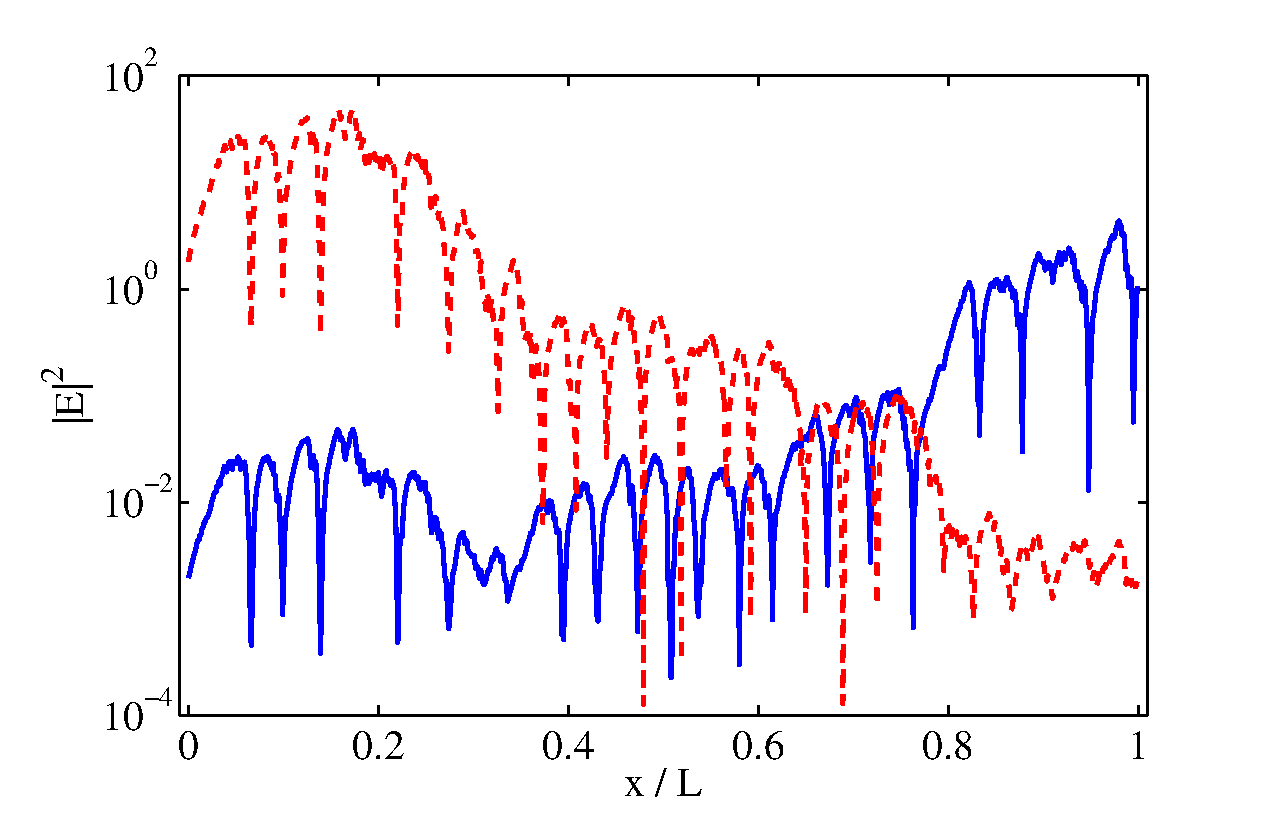
\includegraphics{pictures/alpha_beta_electric_field}}
\scalebox{0.3}{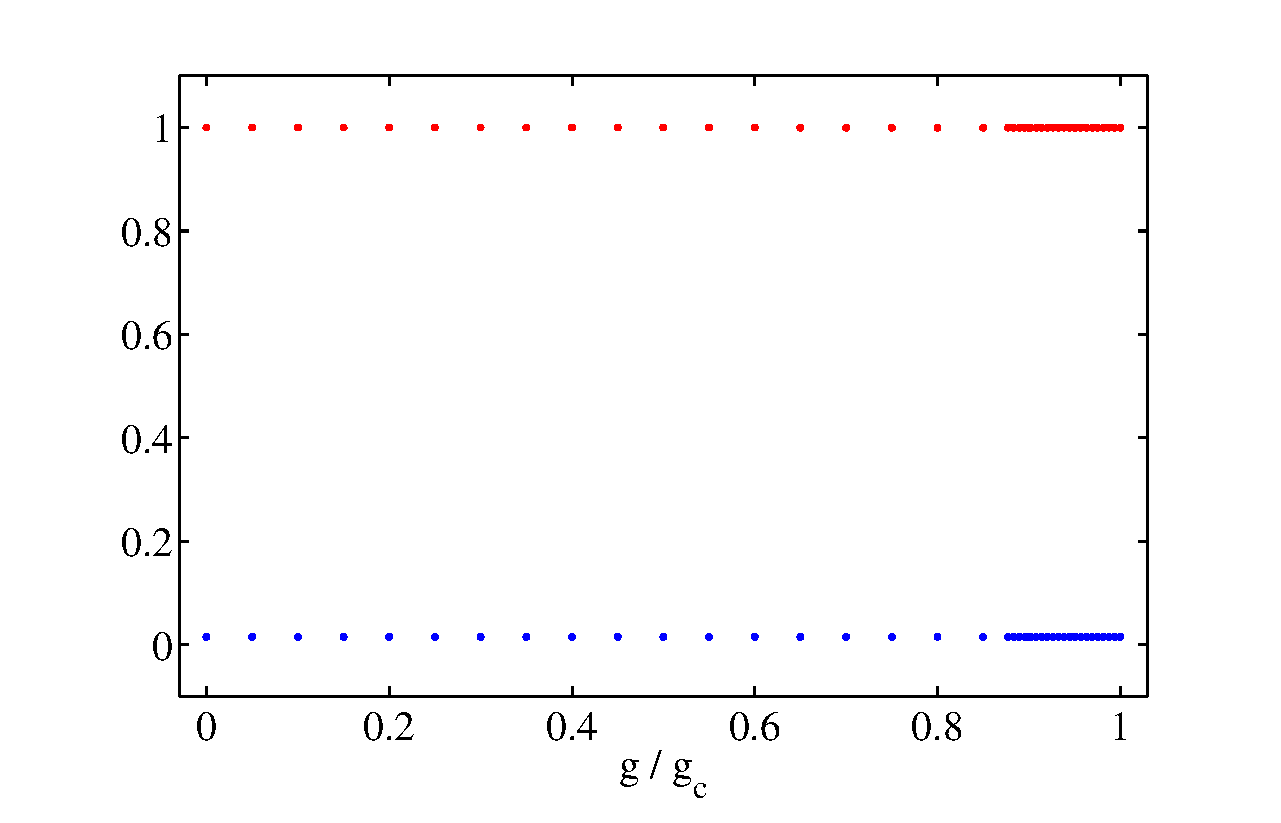
\includegraphics{pictures/alpha2_beta2}}
\scalebox{0.3}{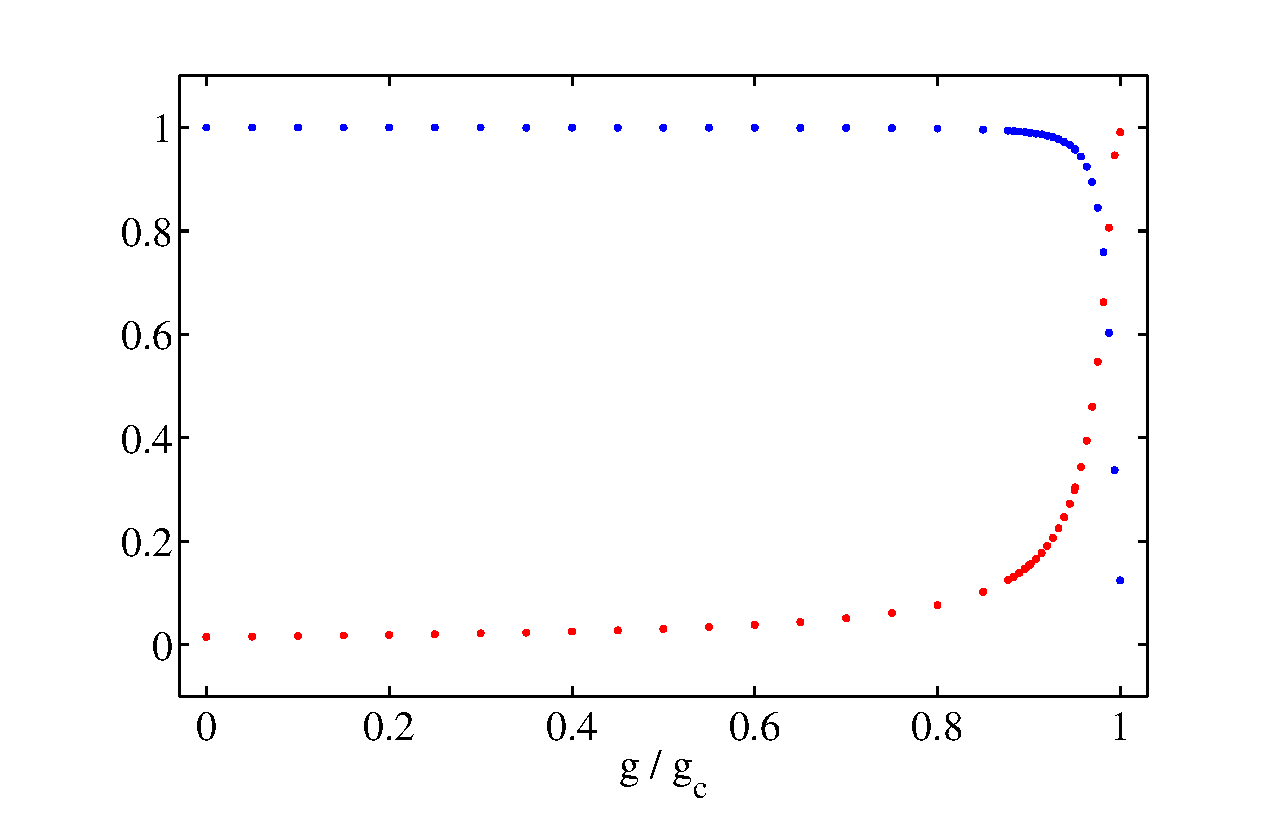
\includegraphics{pictures/alpha1_beta1}}}
%\scalebox{0.5}{\includegraphics{pictures/alpha_beta_reality_check}}}
\vskip -0.5cm
\caption[The left most plot is the electric field for a resonant frequency (blue shows a center of localization at $ \frac{1}{4} $L and is the LR orientation while red shows a center of localization at $ \frac{3}{4} $L and is the RL orientation.]{The left most plot is the electric field for a resonant frequency (blue shows a center of localization at $ \frac{1}{4} $L and is the LR orientation while red shows a center of localization at $ \frac{3}{4} $L and is the RL orientation. The other two plots are the alpha and beta coefficients scanning gain from  passive to critical gain at a resonant frequency for the two orientations. The center is LR and the right is RL. The crossover takes place very near critical gain. This explains why the amount of gain added is more sensitive near critical gain.}
\label{fig:alphabeta}
\end{figure}

What we get from these two plots in Fig.~\ref{fig:alphabeta} is that the two wave functions from the passive system are added up to get the wave form with gain, $ \tilde{\psi}$. The coefficients $\alpha$ and $\beta$ tell how much of each passive waveform to add. In the case of a wave function with center of localization at $ \frac{1}{4} $L there is hardly any contribution from the wave function with center of localization at $ \frac{3}{4} $L, so $\alpha$ and $\beta$ remain at their original 0 and 1 values. For the other canonical case $\alpha$ starts with hardly any contribution to $ \tilde{\psi}$ but as gain is added $\alpha$ dominates.

%%%%%%%%%%%%%%%%%%%%%%%%%%%%%%%%%%%%%%%%%%%%%%%%%%%%%%%%%
\subsection {Summary}
%%%%%%%%%%%%%%%%%%%%%%%%%%%%%%%%%%%%%%%%%%%%%%%%%%%%%%%%%

We were interested in finding a criteria for localization in media with gain.  We suspected the ratio of transmission and energy may be a good parameter.

The analytical diffusion model was the first thing we investigated.  Even though localization could not be present the diffusion equation demonstrated that T/${\cal E}$ was not divergent at the lasing threshold (even though transmission and energy both diverged). 

Next we created a computational model in Fortran for random layers of dielectric.  In this system there is no diffusion and localization does occur.  We used the transfer matrix method to propagate light using Maxwell's equations and recorded transmission, reflection, and electric field in the sample, (total energy in the sample).

Starting in the passive model we see that T/${\cal E}$ is neither smooth nor constant due to peaks in transmission that lack a corresponding peak in energy.  We then determined why this was occurring.  The electric field in the sample at that specific frequency lead us to show that localization is wave ``tunneling'' though the medium. We explain this by looking at two analytical models, the double barrier potential with varying well position and the periodic structure with a single defect. Now we know why there are peaks in transmission but not always energy. This explains why T/${\cal E}$ is not smooth.

Adding gain to the system makes T/${\cal E}$ smoother and it is a good parameter (in that it does not diverge) but T/${\cal E}$ is not constant due to the center of localization varying in the sample for different frequencies.

Flipping the sample and keeping the light that shines on the sample in the original orientation moves the center of localization to the opposite side. This is equivalent to keeping the sample fixed and flipping the light source orientation (now the light shines on the x=L side).

This change in boundary conditions (where the light is shined from) leads to insight on why the waveform of the electric field changes.  Reciprocity in the passive system allows us to construct two waveforms that constitute a basis, similar to the closed system and looking for eigenstates.  Adding gain to the system we use $\psi _1 $ and $\psi _2 $ as the basis.  We use coefficients $\alpha$ and $\beta$ to build the resultant waveform.

\begin{comment}

%%%%%%%%%%%%%%%%%%%%%%%%%%%%%%%%%%%%%%%%%%%%%%%%%%%%%%%%%
\subsection {Future work}
%%%%%%%%%%%%%%%%%%%%%%%%%%%%%%%%%%%%%%%%%%%%%%%%%%%%%%%%%

Now that we understand localization in systems with gain
we will go back and look at passive systems as a limit that
gain goes to zero.

We plan to investigate quasi 1-D systems,
then 2-D, and then 3-D. We should be able to verify that the
same ideas apply from the 1-D system.  Note that the 1-D potential
well extends easily to 2-D and 3-D, in that the boundary
conditions for the 1-D quantum mechanical potential well
are that the wave form is zero at the edges
of the well.

\end{comment}

\newpage
%\begin{appendices}
%%%%%%%%%%%%%%%%%%%%%%%%%%%%%%%%%%%%%%%%%%%%%%%%%%%%%%%%%
\subsection {Medium creation}
%%%%%%%%%%%%%%%%%%%%%%%%%%%%%%%%%%%%%%%%%%%%%%%%%%%%%%%%%
On first inspection, creating a media filled with random scatterers
seems a trivial task.  This is true for low density, as one simply
picks random positions and ensures that no two scatterers are too
close to each other.  However, localization occurs in high-density
scatterers.  There exists a maximum number of spheres that fits in a 
given volume, and as this upper limit is reach it becomes harder
to find the last available volumes to put the scattering sphere in.
For randomly positioned scatterers the upper limit is not well 
defined (realization specific), as the space between scatterers is not constant.

The initial algorithm implemented in code placed a scatterer in the medium by
choosing x,y,z from a uniformly random distribution. If the new position
conflicts with a previously choosen scatterer (distance between scatterers
is too small) then another choice of x,y,z is made. This process is repeated
until a valid scatterer position is found.  The number of unsuccessful 
choices grows with the number of total scatterers for a given volume as
$ ? $

To reduce this problem alternative algorithms were developed.

Instead of attempting to generate a random media, start with a 
lattice of scatterers and then let the scatterers take a random
walk.  However, this results on average that each scatterer is roughly
in the same place it started, a lattice.

Another option was to use a lattice and then allow the scattering
strength $\alpha$ to be random.  This is computationally simple but
introduces ?? band gap effects.

Breaking the medium into smaller containers

Stacking scatterers in the x direction. $\Delta x$ is not uniform, so
the distribution for choosing x,y,z was found.

\newpage
%\begin{appendices}
%%%%%%%%%%%%%%%%%%%%%%%%%%%%%%%%%%%%%%%%%%%%%%%%%%%%%%%%%
\subsection {propagation alternatives}
%%%%%%%%%%%%%%%%%%%%%%%%%%%%%%%%%%%%%%%%%%%%%%%%%%%%%%%%%
For 1D and quasi1D the incident light is a plane wave.  Using self-embedding
technique the eigen values numerical error in the transfer matrix was limited.
However, for certain parameters with quasi-1D the error prevented full investigation.

An alternative to plane wave is ray tracing, which introduces a different set
of complications. Instead of numerical inaccuracy, which can not be overcome, the 
difficulty is computational time. Individual photons are propagated through the 
medium, and a large number of photons is needed. There is error introduced in 
a discrete incident wave.  Even with a large number of incident photon paths, 
there exists the possibility of a path not being taken, since not all y-z choices 
are used.  Normally that would be acceptable, but localization demands that all 
paths be taken, less the one not taken results in the closed path.  By 
ignoring any path, we disregard a small number of localization occurrences.  
A finite number of incident photons ignores an infinite number of path possibilities.
The plane wave, continuous in y-z, takes all paths but error can build up in
the numerical accuracy of the transfer matrix eigenvalues.


\begin{comment}

useful sites for latex formatting
http://en.wikibooks.org/wiki/LaTeX/Mathematics
http://www.tex.ac.uk/cgi-bin/texfaq2html?label=appendix

********************************
conventions:

Fig.~\ref{fig:

Eq.~\ref{fig:

Ref.~\cite{

********************************

version history:

20080514
-changed energy from \xi to {\cal E}
-changed localization length from \zeta to \xi

20080506
-changed localization length \xi to \zeta
-added symbols appendix
-converted from pdf pictures to eps. Now run "latex" instead of "pdflatex"

20080421
-added hyperlinks
-changed energy E to \xi

\end{comment}



